%%%%%%%%%%%%%%%%%%%%%%%%%%%%%%%%%%%%%%%%%%%%%%%%%%%%%%%%%%%%%%%%%%%%%%
% LaTeX Example: Project Report
%
% Source: http://www.howtotex.com
%
%%%%%%%%%%%%%%%%%%%%%%%%%%%%%%%%%%%%%%%%%%%%%%%%%%%%%%%%%%%%%%%%%%%%%%


%%% Preamble
\documentclass[paper=a4, fontsize=12pt]{scrartcl}
\usepackage[T1]{fontenc}
\usepackage{fourier}

\usepackage[utf8]{inputenc}
\usepackage{polski}
\usepackage[protrusion=true,expansion=true]{microtype}	
\usepackage{amsmath,amsfonts,amsthm} % Math packages
\usepackage[pdftex]{graphicx}	
\usepackage{float}
\usepackage{url}
\usepackage[margin=2.5cm]{geometry}
\usepackage{pdfpages}


%%% Custom sectioning
%\usepackage{sectsty}
%\allsectionsfont{\normalfont\scshape}


%%% Custom headers/footers (fancyhdr package)
\usepackage{fancyhdr}
\pagestyle{fancyplain}
\fancyhead{}											% No page header
\fancyfoot[L]{}											% Empty 
\fancyfoot[C]{}											% Empty
\fancyfoot[R]{\thepage}									% Pagenumbering
\renewcommand{\headrulewidth}{0pt}			% Remove header underlines
\renewcommand{\footrulewidth}{0pt}				% Remove footer underlines
\setlength{\headheight}{13.6pt}
\setlength{\parindent}{0pt}
\setlength{\parskip}{10pt}


%%% Equation and float numbering
\numberwithin{equation}{section}		% Equationnumbering: section.eq#
\numberwithin{figure}{section}			% Figurenumbering: section.fig#
\numberwithin{table}{section}				% Tablenumbering: section.tab#


\newcounter{UCCounter}
\newenvironment{usecase}[1]{\paragraph{UC\ifnum\value{UCCounter}<10 0\fi\arabic{UCCounter} #1} \stepcounter{UCCounter} \ \\}

%%% Maketitle metadata
\newcommand{\horrule}[1]{\rule{\linewidth}{#1}} 	% Horizontal rule

\title{
		%\vspace{-1in} 	
		\usefont{OT1}{bch}{b}{n}
		\normalfont \normalsize \textsc{Akademia Górniczo Hutnicza} \\ [25pt]
		Wydział Informatyki, Elektroniki i Telekomunikacji
		\horrule{0.5pt} \\[1cm]
		
\includegraphics[width=.35\textwidth]{img/agh_znk_wbr_cmyk.eps} \\[1.5cm]
		\huge System usprawniający deklarację i zbiórkę odpadów
		\horrule{0.5pt} \\[0cm]
}
\author{
		\normalfont \normalsize
        Mateusz Kwiecień\\[-3pt]	\normalsize
        Beata Obrok\\[-3pt]			\normalsize
        Arkadiusz Socha\\[-3pt]		\normalsize
        Dawid Suder\\[-3pt]			\normalsize
}
\date{}


%%% Begin document
\begin{document}
\maketitle
\tableofcontents
\clearpage

\section{Sformułowanie zadania projektowego}

	\subsection{Obszar i przedmiot modelowania}

		\subsubsection{Dziedzina problemu}
			
% Firma, cel, dziedzina, schemat struktury organizacyjnej, słownik pojęć biznesowych (lub odsyłacz do załącznika)
% Ogólne omówienie zakresu i charakteru działalności jednostki dla której przeznaczony jest produkt tj. realizowany [projektowany] system).
% Dołączyć i opisać schemat struktury organizacyjnej jednostki. 

\paragraph{Wstęp}
\textbf{BIOSYSTEM S.A.} działa jako spółka matka konsolidująca grupę firm działających w sektorze ochrony środowiska i gospodarki odpadami. Spółka pełni funkcję dostarczyciela kapitału, inkubatora projektów w ramach grupy oraz zapewnia współdziałanie poszczególnych podmiotów funkcjonujących na równoległych rynkach.

\paragraph{Zakres i charakter działalności spółki}

Pierwszym przedmiotem działalności spółki jest nadzór właścicielski nad dwoma organizacjami odzysku wspierającymi przedsiębiorców w zakresie realizacji ustawowych obowiązków zbiórki, recyklingu i odzysku odpadów opakowaniowych, zużytych baterii oraz sprzętu elektrycznego i elektronicznego.

Kolejnym, bardzo ważnym, przedmiotem działalności BIOSYSTEM S.A. jest zbiórka, przetwarzanie i unieszkodliwianie zużytego sprzętu elektrycznego i elektronicznego (ZSEiE). Spółka ta prowadzi również najnowocześniejszy w Polsce Zakład Przetwarzania ZSEiE ze specjalną linią do utylizacji urządzeń chłodniczych. Rezultatem tego jest sprzedaż produktów i surowców powstałych w wyniku przetworzenia.

BIOSYSTEM S.A. zajmuje się również importem urządzeń elektrycznych i elektronicznych. W związku z tym prowadzi także sprzedaż detaliczną i hurtową takiego sprzętu.

Ostatnim przedmiotem działalności jest organizacja publicznych kampanii edukacyjnych wykonywanych na zlecenie spółek zależnych.

	\subsection{Obszar modelowania}

		\subsubsection{Opis struktury organizacyjnej}
			
% Opisowy model stanu istniejącego
% Opis wszystkich składników organizacyjnych
% Związek struktury z dziedziną obszaru modelowania, wyznaczenie zakresu odpowiedzialności systemu 	

\paragraph{Grupa Kapitałowa Biosystem} składa się z trzech podmiotów gospodarczych:
\begin{itemize}
	\item \emph{BIOSYSTEM S.A.}
	\item \emph{BIOSYSTEM Elektrorecykling Organizacja Odzysku Sprzętu Elektrycznego i Elektronicznego S.A.}
	\item \emph{Zakład Gospodarki Komunalnej Organizacja Odzysku BIOSYSTEM S.A.}
\end{itemize}
Firma \emph{BIOSYSTEM S.A.} stanowi spółkę nadrzędną.

\begin{figure}[H]
	\centering
	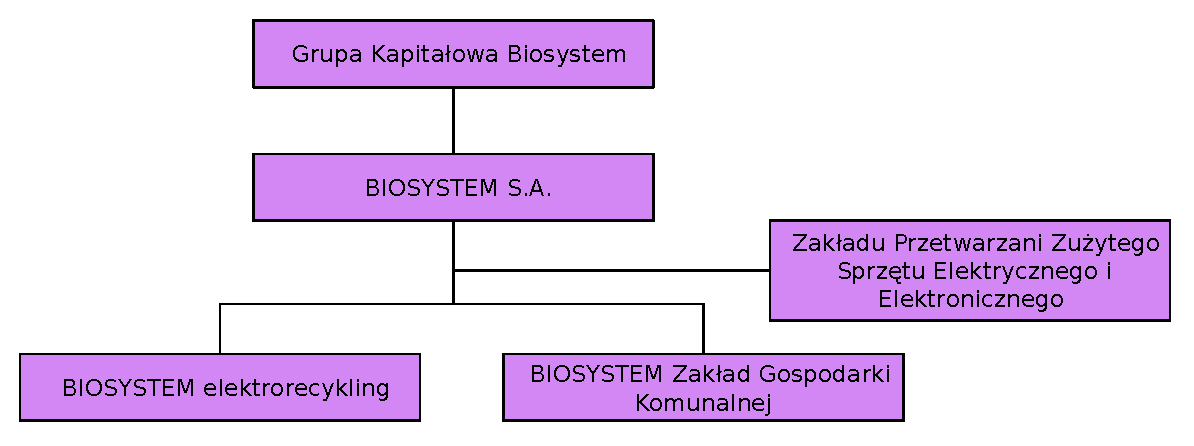
\includegraphics[width=\textwidth]{img/group_chart.eps}
	\caption{Struktura grupy kapitałowej}
\end{figure}

\paragraph{Opis składników organizacyjnych} \ \\
Dwa z tych podmiotów zajmują się sprawozdawczością wobec Urzędów Marszałkowskich zgodnie z ustawą o odpadach.

W ramach działalności współpracują z klientami wprowadzającymi różnego rodzaju materiały do środowiska, które powinny podlegać recyklingowi. W związku z tym prowadzą działalność dodatkową polegającą na zbieraniu opakowań z papieru, tworzyw sztucznych, szkła, blachy i aluminium oraz sprzętu elektrycznego i elektronicznego.

Spółka BIOSYSTEM S.A. jest również właścicielem \emph{Zakładu Przetwarzania Zużytego Sprzętu Elektrycznego i Elektronicznego}, który zajmuje się recyklingiem sprzętu elektrycznego i elektronicznego. 

\paragraph{Odpowiedzialność poszczególnych spółek} \ \\
\begin{enumerate}
	\item \emph{BIOSYSTEM S.A.}: 
		\begin{itemize}
			\item działalność handlowa
			\item nadzór właścicielski nad spółkami zależnymi
		\end{itemize}
	\item \emph{BIOSYSTEM elektrorecykling}: sprawozdawczość w zakresie wprowadzania sprzętu elektrycznego i elektronicznego przez swoich klientów
	\item \emph{BIOSYSTEM ZGK}:
		\begin{itemize}
			\item sprawozdawczość w zakresie wprowadzania opakowań i baterii przez swoich klientów
			\item organizacja przetwarzania opakowań przy pomocy firm współpracujących
		\end{itemize}
\end{enumerate}

\paragraph{Wewnętrzna struktura organizacyjna} \ \\

\begin{figure}[H]
    \centering
    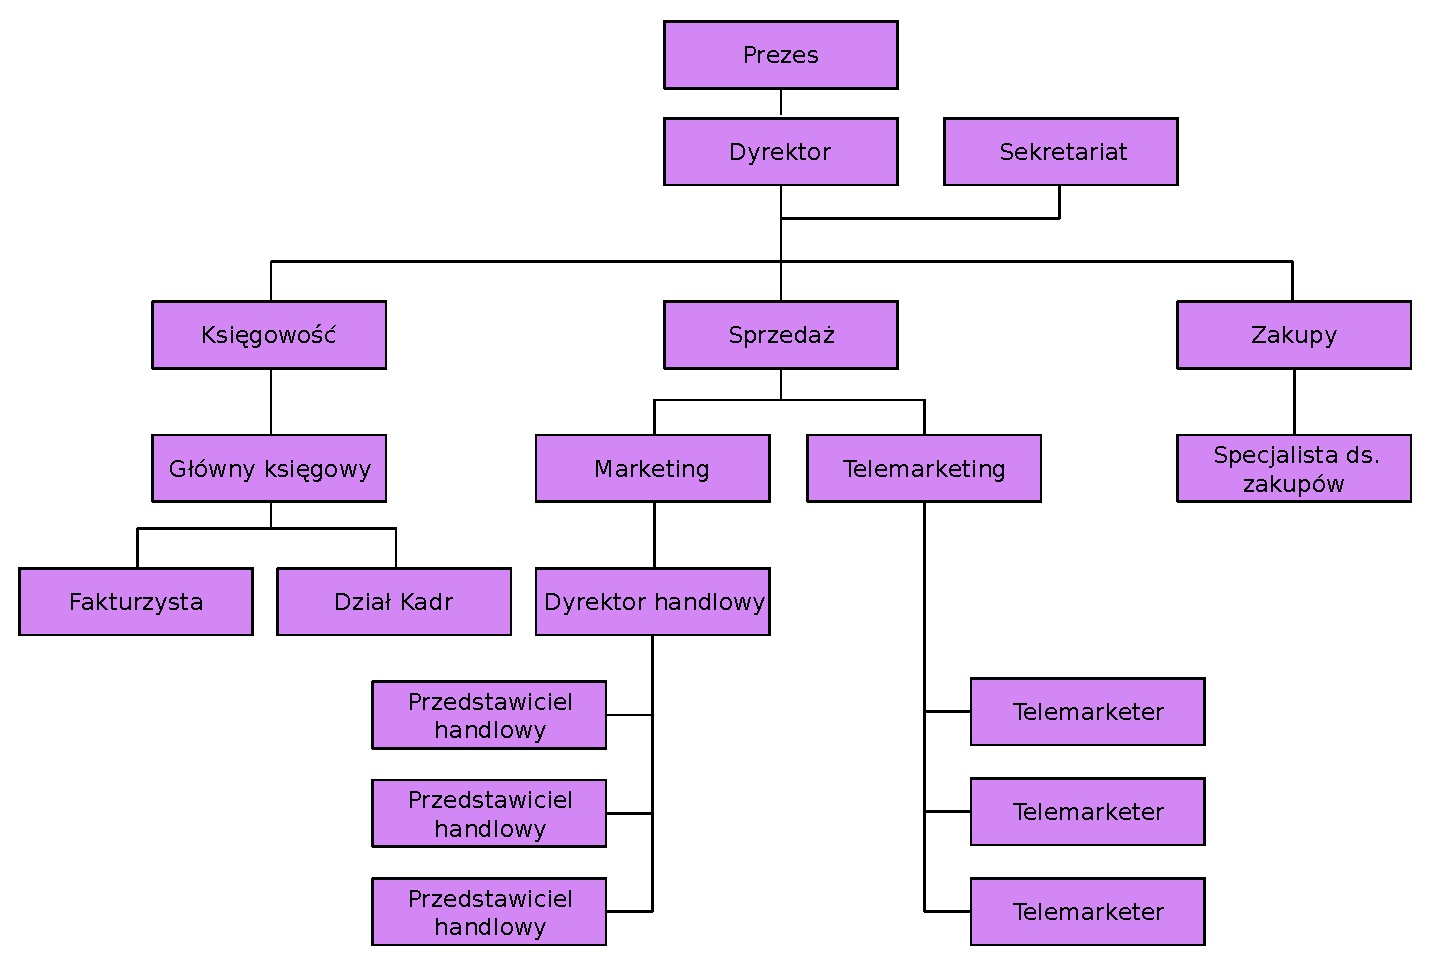
\includegraphics[width=1\textwidth]{img/organization_chart.eps}
    \caption{Struktura organizacyjna spółki}
\end{figure}

		\subsubsection{Obszary aktywności}
			
% Wyznaczenie obszarów aktywności, które będą omówione szczegółowo w kolejnym podrozdziale

\begin{enumerate}
	\item Obsługa oddającego odpady \\
	W zależności od ilości odpadów, a także od lokalizacji klienta, firma może wysłać kierowcę po ich odbiór, lub sprzedający może przywieźć je osobiście.
	\item Obsługa kupującego \\
	Kupujący składa zamówienie osobiście, telefonicznie, a także za pomocą strony internetwowej. Firma wysyła kierowcę z zamówieniem, a klient odpbiera je płacąc, za dowieziony towar, chyba, że wcześniej zapłacił za niego przelewem.
	\item Wspomaganie pracy kierowców \\
	Kierowcy odbierają odpady od klientów z terenów Małopolski. Zabierają ze sobą potwierdzenie odbioru, którą wręczają sprzedającemu. Następnie przewożą odpady do:
		\begin{itemize}
			\item zewnętrznej firmy recyklingowej(opakowania z papieru, tworzyw sztucznych, szkła, blachy i aluminum),
			\item własnego zakładu przetwarzania sprzętu elektrycznego i elektronicznego.
		\end{itemize}
	Kierowcy zajmują sie także dostarczeniem zamówienia do kupującego. Zabierają ze sobą fakturę, którą wręczają kupującemu.
	\item Wspomaganie pracy magazynierów \\
	Pracownicy magazynu grupują produkty otrzymane po recyklingu. Zajmują się także przygotowaniem 
	\item Wspomaganie pracy pracownika działu sprzedaży \\
	Dział sprzedaży zajmuje się pozyskiwaniem klientów, którzy kupią odpady poddane już recyklingowi. Dział ten zajmuje także obsługą klienta, który składa deklaracje o ilości odpadów, które ma do sprzedania. Deklaracje mogą być składane poprzez stronę internetową, a dział sprzedaży sprawdza ich poprawność.
\end{enumerate}


	\subsection{Opis obszarów aktywności}

		\subsubsection{Opis stanowisk pracy}
			
\begin{enumerate}
	\item Właściciel \\ 
	Właściciel firmy odpowiada za jej funkcjonowanie, podlegają mu pracownicy. Do jego głównych zadań należą:
	\begin{itemize}
		\item organizacja pracy podwładnych i ustalanie wynagrodzenia
		\item nadzór nad spółkami zależnymi
	\end{itemize}
	\item Pracownik działu odbioru \\
	Przygotowują potwierdzenia odbioru, oraz przekazanie je kierowcy. Zajmują się także skupem oświadczeń oddzysku.
	\item Pracownicy działu sprzedaży
	\begin{itemize}
	\item Pracownik działu sprzedaży\\
	Zajmuje się pozyskiwaniem nowych klientów odwiedzając placówki firm potencjalnie zainteresowanych usługami naszej firmy, zajmują się też odbieraniem deklaracji ilości odpadów od sprzedającego
	\item Telemarkter \\
	Zajmuje się pozyskiwaniem nowych klientów dzwoniąc do firm potencjalnie zainteresowanych usługami naszej firmy.
	\end{itemize}
	\item Magazynier \\
	Do jego głównych zadań należą:
		\begin{itemize}
		\item oprzygotowanie zamówień
		\item odbieranie dostaw od kierowców
		\item aktualizacja stanu magazynu
		\end{itemize}
	\item Kierowca \\
	Odbiera odpady od sprzedających, przewozi je do miejsc, gdzie są poddawane recyklingowi. Przewozi także produkty recyklingu do magazynu, a także zawozi je do kupującego.
	\item Księgowy \\
	Zajmuje się wystawianiem faktur, tworzeniem raportów finansowych oraz rozliczenianiem firmy z urzędem skarbowym.
\end{enumerate}



		\subsubsection{Opis procedur biznesowych}
			
\begin{enumerate}
	\item Obsługa klienta
		\begin{itemize}
			\item złożenie deklaracji o ilości odpadów \\
			Klient podaje informacje o rodzaju oraz ilości (lub wadze) odpadów, które wprowadził do obiegu w danym okresie rozliczeniowym poprzez formularz udostępniany przez system. Dane dotyczące deklaracji zostają zapisane w \emph{rejestrze deklaracji}.
			\item oddanie odpadów \\
			Klient za pomocą formularza udostępnianego przez system zamawia kierowcę do odbioru odpadów przeznaczonych do odsyku.
			Dane dotyczące odpadów oraz adres odbioru zostają zapisane w \emph{rejestrze ofert sprzedaży}
			\item złożenie zamówienia
			Klient za pomocą formularza udostępniane przez system wprowadza surowce, które chce zamówić, oraz adres dostawy. Dane o zamówienia zostają zapisane w \emph{rejestrze zamówień}
		\end{itemize}

	\item Obsługa skupu
		\begin{itemize}
			\item przetworzenie oferty sprzedaży \\
			Pracownik sprawdza możliwość odbioru odpadów oraz przydziela placówkę, do której należy przewieźć odpady.
			\item zakup oświadczenia odzysku \\ 
			Pracownik na podstawie deklaracji klientów zamawia w zewnętrznym zakładzie przetwarzania oświadczenia odzysku oraz odbiera fakturę za wykonany recykling.
		\end{itemize}

	\item Obsługa kierowców 
		\begin{itemize}
			\item przydzielenie kierowcy do zlecenia \\
			Kierowca otrzymuje informacje o adresie klienta.
			\item odebranie towaru z magazynu 
			\item dostarczenie towaru do klienta
			\item odbiór odpadów od klienta
			\item dostarczenie surówców wtórnych do placówek recyklingowych \\
			Kierowca dostarcza odpady, do odpowiednich placówek, pobiera potwierdzenie odbioru.
		\end{itemize}

	\item Obsługa magazynu
		\begin{itemize}
			\item aktualizacja stanu magazynu \\
		 	Magazynier uaktualnia ilość poszczególnych produktów, modyfikując rejestr stanu magazynu.
		 	\item przygotowanie towaru do sprzedaży \\
		 	Magazynier dostaje informacje o zamówieniu(poprzez rejestr zamówień), które kompletuje.
		\end{itemize}

	\item Obsługa księgowości
		\begin{itemize}
			\item generowanie faktur \\ 
			Generowanie faktur na podstawie danych zawartych w rejestrach zamówień. System zapisuje je w rejestrze faktur.
			\item wprowadzanie faktur \\
			Wpraowadzanie do systemu faktur, które firma otrzymuje przy zakupie oświadczeń oddzysku.
		\end{itemize}

	\item Wspomaganie pracy właściciela
		\begin{itemize}
			\item generowanie raportów przychodów i wydatków\\
			System generuje wyżej wymienione raporty, na podstawie danych zawartych w rejestrze faktur. Raporty są zapisywane w rejestrze raportów.
			\item generowanie raportów aktywności klientów \\
			System generuje raport na podstawie rejestrów deklaracji i zamówień.
		\end{itemize}

\end{enumerate}

	\subsection{Zakres odpowiedzialności systemu}
		
% Szczegółowe wyznaczenie, jaka część obszaru modelowania będzie [lub jest] objęta funkcjami realizowanymi przez opracowywany system).
% Model (opisowy) stanu istniejącego powinien uwzględniać charakterystykę wyodrębnionych „obszarów aktywności” systemu
% (podsystemów) oraz bardzo szczegółowy opis procedur biznesowych. Stanowią one podstawę do konstrukcji (lub są nimi) biznesowych
% przypadków użycia, a następnie systemowych przypadków użycia. Uzupełnić słownikiem pojęć biznesowych 
% (zamieszczonym w Dodatku, referencje w tekście) 

W zakres odpowiedzialności systemu wchodzą wszystkie procedury z pkt 1.3.
Główną odpowiedzialnością naszego systemu jest zarządzanie strukturą firmy, pomoc 
w zautomatyzowaniu niektórych aktywności, które teraz wykonywane są ręcznie np. przesyłanie dokumentów 
pomiędzy sektorami firmy (zamówienie -> kierowca), kontrola stanu magazynu, kontrola stanu "przesyłki".


	\subsection{Zwięzła nazwa problemu}
		
% Jednozdaniowa pełna nazwa [tytuł] przedsięwzięcia wraz z krótkim uzasadnieniem jej wyboru oraz nazwa kodowa 
% [„kryptonim”, jedno % dwa słowa, mogące stanowić nazwę własną produktu].

\emph{System usprawniający deklarację i zbiórkę odpadów} 

System ma umożliwiać firmom internetową deklarację wprowadzanych odpadów oraz usprawniać przepływ informacji i organizację przewozu odpadów pomiędzy składowymi spółkami grupy Biosystem oraz zewnętrznymi firmami przetwarzającymi odpady.

\paragraph{Nazwa kodowa} \textbf{iRecykling}

	\subsection{Cele do osiągnięcia}

		\subsubsection{Cele produktu}
			
% Cele z punktu widzenia użytkownika końcowego lub zleceniodawcy oraz cele dodatkowe – dołączone przez jednostkę
% projektującą [firmę projektową, zespół projektantów], zwykle dotyczą specyficznych, niewidocznych dla użytkownika 
% cech realizowanego systemu, np. związane z zarządzaniem systemem, bezpieczeństwem, itp.

Zadaniem zespołu projektowego jest stworzenie systemu umożliwiającego składanie klientom firmy BIOSYSTEM deklaracji on-line niezbędnych do stworzenia sprawozdań dla Urzędów Marszałkowskich zgodnie z ustawą o odpadach oraz usprawniający proces obsługi deklaracji i zbiórki odpadów oraz przewozu odpadów do placówek zajmujących się ich utylizacją.

Proces składania deklaracji powinien być intuicyjny i możliwie najmniej skomplikowany. Zespół będzie musiał zadbać o to, aby pobrać wszystkie niezbędne informacje możliwie najbardziej przyjazny sposób. Istotne jest także, żeby informacje te, były dostarczone do docelowego klienta w formie wygodnej do dalszego wykorzystania.

Istotne jest również bezpieczeństwo systemu i danych osobowych klientów. 

		\subsubsection{Cele przedsięwzięcia projektowego}
			
% Cele stawiane przed zespołem projektowym, nieistotne lub drugorzędne dla zleceniodawcy albo wręcz nie ujawniane przed nim; 
% przeważnie dotyczą one sposobu prowadzenia przedsięwzięcia projektowego [np. stosowane metodyki, narzędzia] lub pobocznych, 
% niewidocznych dla użytkownika i zleceniodawcy systemu efektów procesu jego wytwarzania, np. [dodatkowy opis, wskazówki, instrukcje]

Celem przedsięwzięcia projektowego jest zapoznanie się z technikami i narzędziami wykorzystywanymi do Projektowania Systemów Informatycznych, jak i naukę pracy grupowej.

Wynikiem tych działań ma być szczegółowy projekt Systemu dla danego problemu, w naszym przypadku zaprojektowanie struktury firmy BIOSYSTEM, który pokaże nam w praktyczny sposób konieczność tych działań. Projekt jest bazowany na realnym problemie, dlatego też pomoże nam to wyrobić pewne, bardziej praktyczne niż teoretyczne, nawyki.


\section{Opis wymagań}
	% Uwaga 1: na tę część opracowania składają się głównie notatki z
	% wywiadów prowadzonych przez analityków, wyniki analizy dokumentów
	% stosowanych w informatyzowanej jednostce, rezultaty ankietowych badań
	% opinii wybranych, kompetentnych pracowników jednostki itp.

	% Uwaga 2: dla większości systemów rozmiar tej części jest na tyle duży, że
	% większość materiału (z wyjątkiem niektórych wyników ustaleń,
	% podsumowania i wniosków) zostaje wyłączona z głównej części
	% opracowania projektowego i przeniesiona do Dodatków, łącznie z przykładami
	% dokumentów źródłowych i innymi, nie włączonymi do ostatecznej
	% wersji dokumentacji projektowej fragmentami opracowania [„nic, co
	% napisane a nie fałszywe, nie powinno zostać wyrzucone”]. 

	\subsection{Funkcje systemu z punktu widzenia użytkownika}
		% zebrane wymagania funkcjonalne, mogą zostać opisane przy pomocy
% formularzy opisu wymagań funkcjonalnych

\begin{enumerate}

\item Funkcje systemu z punktu widzenia Klienta:
	\begin{itemize}
		\item Dodaj deklarację
		\item Modyfikuj deklarację
		\item Wyświetl szczegółowe informacje na temat deklaracji
		\item Wyświetl listę deklaracji
		\item Zleć odbiór odpadów
		\item Zamów surowce
	\end{itemize}

\item Funkcje systemu z punktu widzenia Pracownika działu sprzedaży:
	\begin{itemize}
		\item Dodaj klienta do bazy danych
	\end{itemize} 

\item Funkcje systemu z punktu widzenia Pracownika działu skupu:
	\begin{itemize}
		\item Wyświetl podsumowania deklaracji
		\item Wprowadź oświadczenie odzysku
	\end{itemize}

\item Funkcje systemu z punktu widzenia Księgowego:
	\begin{itemize}
		\item Generuj fakturę sprzedaży produktów recyklingu
		\item Generuj fakturę dotyczącą usługi przejęcia obowiązku recyklingu
		\item Wprowadź dane faktury kupna oświadczeń o przetworzeniu odpadów
		\item Generuj raport przychodów i rozchodów
	\end{itemize}

\item Funkcje systemu z punktu widzenia Magazyniera:
	\begin{itemize}
		\item Przyjmij produkty od magazynu 
		\item Aktualizuj stan magazynu
		\item Kompletuj zamówienie
		\item Wydaj zamówienie
	\end{itemize}

\item Funkcje systemu z punktu widzenia Kierowcy:
	\begin{itemize}
		\item Sprawdź informacje o zamówieniu
		\item Drukuj fakturę dotyczącą zamówienia
		\item Drukuj potwierdzenie odbioru dotyczące zlecenia
		\item Wprowadź potwierdzenie odbioru do systemu
	\end{itemize}

\item Funkcje systemu z punktu widzenia Właściciela:
	\begin{itemize}
		\item Generuj raport przychodów i rozchodów
		\item Generuj raport aktywności klientów
	\end{itemize}

\end{enumerate}


	\subsection{Dane przechowywane w systemie}
		% określony ma zostać ich rodzaj i dołączone wzory-
\begin{enumerate}
	\item Dane klientów(zarówno sprzedających jak i kupujących)
	\begin{itemize}
		\item Nazwa firmy
		\item Adres
		\item NIP
		\item Historia transakcji
		\item Numer telefonu
	\end{itemize}
	\item Dane o ofertach sprzedaży
	\begin{itemize}
		\item Dane o firmie sprzedającego
		\item Dane dotyczące rodzaju odpadów
		\item Ilość poszczególnych rodzajów odpadów
		\item Data deklaracji
		\item Data możliwego odbioru
	\end{itemize}
	\item Dane o deklaracjach
	\begin{itemize}
		\item Dane klienta
		\item Rodzaj odpadów
		\item Ilośc lub waga odpadów
		\item Data deklaracji
	\end{itemize}
	\item Dane o zamówieniach
	\begin{itemize}
		\item Dane o firmie kupującego
		\item Spis produktów recyklingu
		\item Ilość poszczególnych produktów
		\item Data
		\item Status zamówienia
		\item Cena
	\end{itemize}
	\item Dane o potencjalnych klientach
	\begin{itemize}
		\item Nazwa firmy
		\item Numer telefonu
		\item Adres
	\end{itemize}
	\item Dane o stanie magazynu
	\begin{itemize}
		\item Rodzaj produktów recyklingu
		\item Ilość poszczególnych produktów
	\end{itemize}
	\item Dane o pracownikach
	\begin{itemize}
		\item Imie
		\item Nazwisko
		\item PESEL
		\item Data urodzenia
		\item Data zatrudnienia
		\item Stanowisko
		\item Bezpośredni zwierzchnik
	\end{itemize}
	\item Dane o fakturach 
	\begin{itemize}
		\item Dane kupującego i sprzedającego
		\item Informacje o produktach
		\item Ilość poszczególnych produktów
		\item Cena
	\end{itemize}
	\item Dane o raportach 
	\begin{itemize}
		\item Rodzaj raportu
		\item Informacje o zyskach
		\item Informacje o stratach
		\item Potencjalne fundusze na inwestycje po danym okresie
	\end{itemize}
\end{enumerate}

	\subsection{Dokumenty wprowadzane i wyprowadzane z systemu}
		% rodzaje, wzory dokumentów zebranych lub „odtworzonych”

\subsubsection{Dokumenty wprowadzane}

	\paragraph{Dane klienta} $\rightarrow$ Projekt interfejsu 1.1. \\
	Ekstrakt z umowy, która jest dokumentem zewnętrznym systemu (nie jest przechowywana w formie elektronicznej).
	Umowa jest zawarta pomiędzy klientem a firmą BIOSYSTEM i świadczy o przejęciu od klienta obowiązku odzysku odpadów przez firmę BIOSYSTEM.

	Zawiera istotne dane klienta (informacje dot. firmy, zakres świadczonych usług (rodzaje odpadów, okresy rozliczeniowe) oraz dane użytkownika w systemie (nazwa użytkownika i hasło klienta).

	\paragraph{Deklaracja} $\rightarrow$ Załącznik 1.2 \\
	Dokument składany przez \emph{Klienta z umową} dotyczący wprowadzonych do obiegu opakowań, baterii, sprzętu elektrycznego i elektronicznego oraz ich ilości i/lub wagi.

	\paragraph{Oferta sprzedaży} $\rightarrow$ Projekt interfejsu 1.2.\ \\
	Dokument składany w systemie przez osobę prywatną lub firmę dotyczący posiadanych przez klienta odpadów przeznaczonych do odbioru przez firmę BIOSYSTEM oraz późniejszej utylizacji w \emph{Zakładzie Przetwarzania Odpadów}.

	\paragraph{Zlecenie odbioru} \ \\
	Zlecenie generowane na podstawie \emph{Oferty sprzedaży} zawierające adres klienta, który zlecił odbiór odpadów oraz adres placówki do której zawiezione zostaną odpady w celu ich recyklingu.

	\paragraph{Zamówienie} \ \\
	Zamówienie składane przez klienta na surowce pochodzące z \emph{Zakładu Przetwarzania Zużytego Sprzętu Eletrycznego i Elektronicznego BIOSYSTEM SA}.

	\paragraph{Oświadczenie odzysku} \ \\
	Dokument kupowany od \emph{Zewnętrznych Zakładów Przetwarzających Odpady}, który opisuje rodzaje odzyskanych odpadów oraz ich ilości.

	Po przejęciu obowiązku odzysku odpadów od klienta firma BIOSYSTEM zleca \emph{Zewnętrznym Zakładom Przetwarzającym Opady} odzyskanie ilości odpadów odpowiadającym wprowadzonym do obiegu przez klienta.

\subsubsection{Dokumenty wyprowadzane}
	\paragraph{Faktura VAT} $\rightarrow$ Załącznik 1.3 \\
	Faktura wystawiana dla klienta za usługę przejęcia obowiązku recyklingu deklarowanych odpadów lub za zamówione surowce.

	\paragraph{Potwierdzenie odbioru} \ \\
	Dokument podpisywany przez klienta poświadczający odbiór przez kierowcę odpadów przeznaczonych do odzysku.


	\subsection{Wymagania specjalne i ograniczenia}
		% zebrane wymagania niefunkcjonalne; np. co do własności produktu,
% obowiązkowego czasu przechowywania danych archiwalnych, okresowości
% przygotowywania raportów, współpracy z innymi systemami, itp.
% zaklasyfikować do głównych grup: [produktowe, organizacyjne,
% zewnętrzne]

\begin{enumerate}
\item Bezpieczeństwo \\
	W systemie przechowywane są wszystkie dane dotyczące firm współpracujących i pracowników, dlatego też dane powinny być chronione przed nieupoważnionym dostępem.
	Utrata danych, bądź ich kradzież może spowodować duże straty finansowe firmy.
	Dane powinny być często backup'owane.

\item Stabilność \\
	System powinien być dostępny cały czas, a w sytuacji pesymistycznej przynajmniej w czasie pracy biura.
	Brak możliwości korzystania z systemu powoduje opóźnienia w realizacji zamówień i niemożność ich złożenia.

\item Łatwość nauki i obsługi \\
	System musi być na tyle intuicyjne i łatwy w obsłudze, aby nie trzeba było przeznaczać pieniędzy na doszkalanie nowych pracowników.
	Powinien być także funkcjonalny, aby maksymalnie zaoszczędzić czas na najczęściej wykonywane czynności.

\end{enumerate}


% -------------------------------------------------------------------------------

	\subsection{Analiza wymagań funkcjonalnych}
		% diagramy i scenariusze UC
		
\begin{figure}[H]
	\centering
	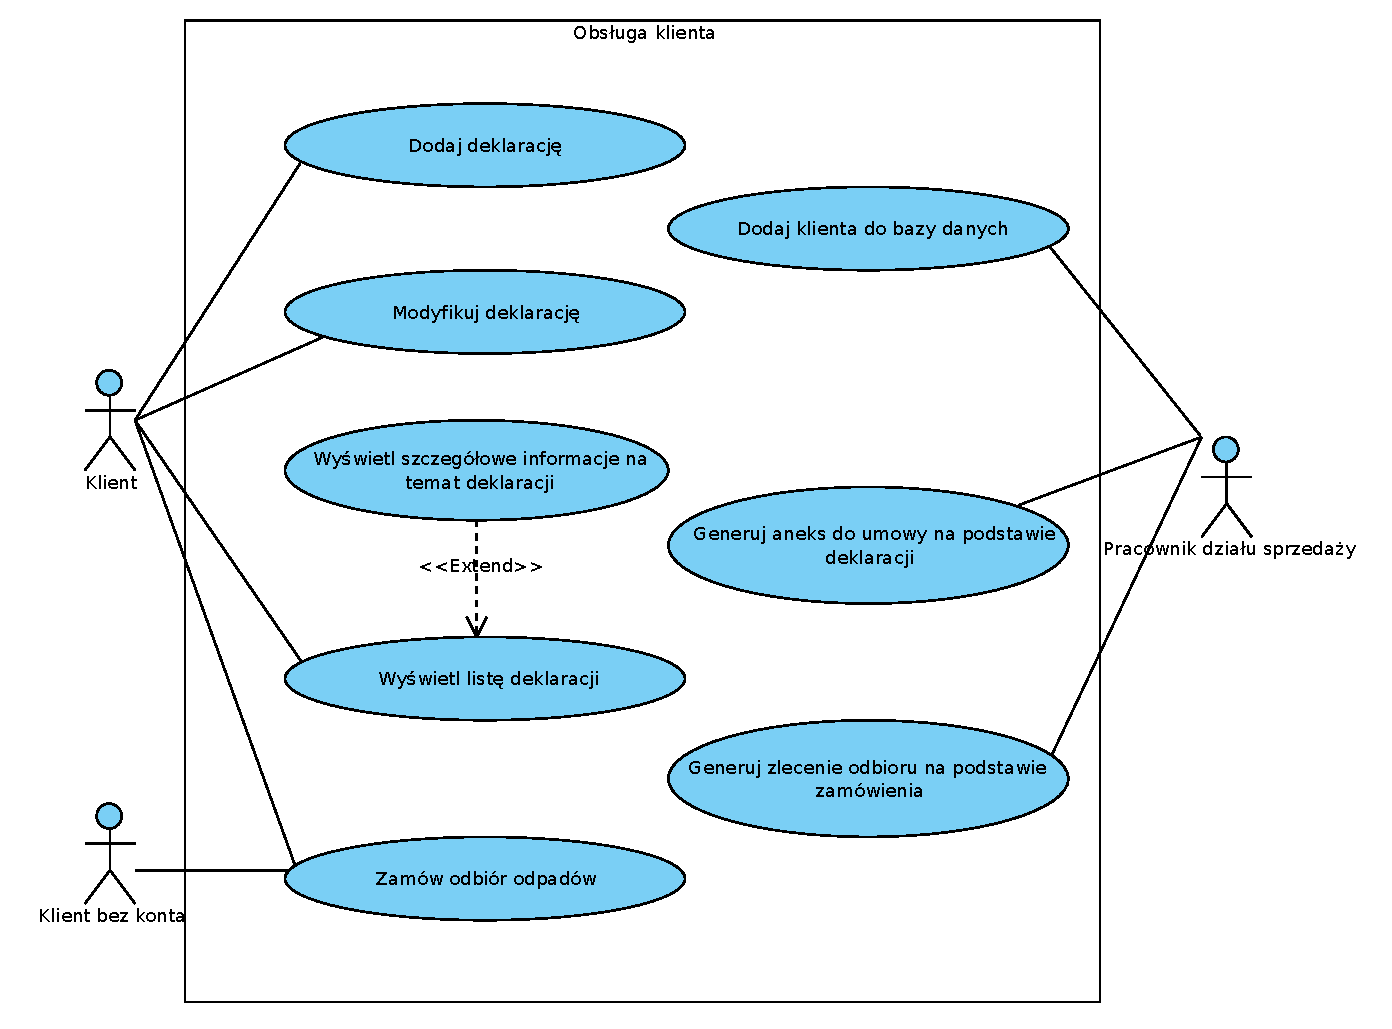
\includegraphics[width=1.1\textwidth]{img/UC/deklaracje.eps}
\end{figure}

\begin{usecase}{Dodaj deklarację}
	\textbf{Autor:} Beata Obrok \\
	\textbf{Cel przypadku użycia:} dodanie deklaracji w celu jej realizacji \\
	\textbf{Kontekst użycia:} chęć dodania deklaracji \\
	\textbf{Zakres:} System obsługi klienta \\
	\textbf{Poziom:} biznesowy \\
	\textbf{Aktor główny:} Klient \\
	\textbf{Wyzwalacz:} wybranie zakładki dodawania deklaracji \\
	\textbf{Warunek początkowy:} klient jest zalogowany i ma uprawnienia do dodawania deklaracji \\
	\textbf{Minimalna gwarancja:} w przypadku nieprzyjęcia deklaracji klient zostanie poinformowany o problemie \\
	\textbf{Główny scenariusz powodzenia:} \\
		\begin{enumerate}
			\item Klient wprowadza rok, na który chce deklarować
			\item Klient poprawnie wybiera miesiące, na które chce deklarować
			\item Klient wybiera kategorię odpadów z listy kategorii
			\item System wyświetla listę odpadów z danej kategorii, które zostały zawarte w umowie z klientem
			\item Klient wybiera odpady, które chce zadeklarować
			\item Klient poprawnie wprowadza ilości i/lub wagi wybranych odpadów
			\item Klient wybiera opcję wysłania deklaracji
			\item System pozytywnie weryfikuje poprawność deklaracji
			\item System zapisuje deklarację w systemie
			\item System wyświetla informację o poprawnym zapisaniu deklaracji w systemie
		\end{enumerate}
	\textbf{Rozszerzenia:} \\
		2.1. Klient wybrał miesiące, na które istnieją już deklaracje \\
			\indent 2.1.1. System wyświetla informację o niemożliwości dodanie deklaracji \\
		4.1. Klient wybiera opcję wyświetlania wszystkich odpadów \\
			\indent 4.1.1. System wyświetla listę wszystkich odpadów z danej kategorii \\
			\indent 4.1.2. Klient wybiera odpady, które chce zadeklarować \\
			\indent 4.1.3. System wysyła informację do opiekuna klienta o potrzebie podpisania aneksu do umowy -> pt 6 \\
		6.1. Klient wprowadza błędną ilość odpadów -> System wyświetla informację o błędnych danych \\
		8.1. System negatywnie weryfikuje poprawność deklaracji -> Wyświetla informację o błędnych danych \\
		10.1. System wyświetla informację o błędzie zapisu do bazy danych \\
\end{usecase}

\begin{usecase}{Wyświetl listę deklaracji}
	\textbf{Autor:} Beata Obrok \\
	\textbf{Cel przypadku użycia:} Wylistowanie deklaracji złożonych przez klienta \\
	\textbf{Kontekst użycia:} chęć przejżenia deklaracji\\
	\textbf{Zakres:} System obsługi klienta \\
	\textbf{Poziom:} biznesowy \\
	\textbf{Aktor główny:} Klient\\
	\textbf{Wyzwalacz:} wybranie zakładki z listą deklaracji \\
	\textbf{Warunek początkowy:} klient jest zalogowany \\
	\textbf{Główny scenariusz powodzenia:} \\
		\begin{enumerate}
			\item System wyświetla deklaracje przypisane do nazwy użytkownika klienta
		\end{enumerate}
\end{usecase}

\begin{usecase}{Modyfikuj deklarację}
	\textbf{Autor:} Beata Obrok \\
	\textbf{Cel przypadku użycia:} Modyfikacja dodanego przez tego klienta deklaracji \\
	\textbf{Kontekst użycia:} chęć modyfikacji istniejącej deklaracji\\
	\textbf{Zakres:} System obsługi klienta \\
	\textbf{Poziom:} biznesowy \\
	\textbf{Aktor główny:} Klient\\
	\textbf{Wyzwalacz:} wybranie przycisku modyfikacji wybranej deklaracji \\
	\textbf{Warunek początkowy:} klient jest zalogowany\\
	\textbf{Minimalna gwarancja:} w przypadku błędu deklaracja pozostanie w stanie oryginalnym \\
	\textbf{Główny scenariusz powodzenia:} \\
		\begin{enumerate}
			\item System wyświetla stronę modyfikacji deklaracji
			\item System wyświetla listę odpadów z kategorii dotyczącej danej deklaracji
			\item Klient wybiera odpady, które chce zadeklarować
			\item Klient poprawnie modyfikuje ilości i/lub wagi wybranych odpadów
			\item Klient wybiera opcję wysłania deklaracji
			\item System pozytywnie weryfikuje poprawność deklaracji
			\item System zapisuje deklarację w systemie
			\item System wyświetla informację o poprawnym zapisaniu deklaracji w systemie
		\end{enumerate}
			3.1. Klient dodaje nowe odpady do deklaracji
				\indent 4.1.1. Klient wpisuje ilości i/lub wagi wybranych odpadów -> pt 5
			3.2. Klient wybiera opcję wyświetlania wszystkich odpadów \\
				\indent 4.1.1. System wyświetla listę wszystkich odpadów z danej kategorii \\
				\indent 4.1.2. Klient wybiera odpady, które chce zadeklarować \\
				\indent 4.1.3. System wysyła informację do opiekuna klienta o potrzebie podpisania aneksu do umowy -> pt 5 \\
			4.1. Klient wprowadza błędną ilość odpadów -> System wyświetla informację o błędnych danych \\
			6.1. System negatywnie weryfikuje poprawność deklaracji -> Wyświetla informację o błędnych danych \\
			8.1. System wyświetla informację o błędzie zapisu do bazy danych \\
\end{usecase}

\begin{usecase}{Wyświetl szczegółowe informacje na temat deklaracji}
	\textbf{Autor:} Beata Obrok \\
	\textbf{Cel przypadku użycia:} Wyświetlenie szczegółów wybranej deklaracji \\
	\textbf{Kontekst użycia:} chęć dostania szczegółowych informacji o deklaracji\\
	\textbf{Zakres:} System obsługi klienta \\
	\textbf{Poziom:} biznesowy \\
	\textbf{Aktor główny:} Klient\\
	\textbf{Wyzwalacz:} wybranie deklaracji z listy deklaracji użytkownika \\
	\textbf{Warunek początkowy:} klient jest zalogowany i ma wyświetloną listę deklaracji\\
	\textbf{Główny scenariusz powodzenia:} \\
		\begin{enumerate}
			\item System wyświetla szczegółowe informacje dotyczące danej deklaracji
		\end{enumerate}
\end{usecase}

% TODO
\begin{usecase}{Zleć odbiór odpadów}
	\textbf{Autor:} Beata Obrok \\
	\textbf{Cel przypadku użycia:} \\
	\textbf{Kontekst użycia:} \\
	\textbf{Zakres:} System obsługi klienta \\
	\textbf{Poziom:} biznesowy \\
	\textbf{Aktor główny:} Klient\\
	\textbf{Wyzwalacz:} \\
	\textbf{Warunek początkowy:} \\
	\textbf{Główny scenariusz powodzenia:} \\
		\begin{enumerate}
			\item
		\end{enumerate}
\end{usecase}

% TODO
\begin{usecase}{Zamów surowce}
	\textbf{Autor:} Beata Obrok \\
	\textbf{Cel przypadku użycia:} \\
	\textbf{Kontekst użycia:} \\
	\textbf{Zakres:} System obsługi klienta \\
	\textbf{Poziom:} biznesowy \\
	\textbf{Aktor główny:} Klient\\
	\textbf{Wyzwalacz:} \\
	\textbf{Warunek początkowy:} \\
	\textbf{Główny scenariusz powodzenia:} \\
		\begin{enumerate}
			\item
		\end{enumerate}
\end{usecase}

% TODO
\begin{usecase}{Dodaj klienta do bazy danych}
	\textbf{Autor:} Beata Obrok \\
	\textbf{Cel przypadku użycia:} \\
	\textbf{Kontekst użycia:} \\
	\textbf{Zakres:} System obsługi klienta \\
	\textbf{Poziom:} biznesowy \\
	\textbf{Aktor główny:} Pracownik działu sprzedaży \\
	\textbf{Wyzwalacz:} \\
	\textbf{Warunek początkowy:} \\
	\textbf{Główny scenariusz powodzenia:} \\
		\begin{enumerate}
			\item
		\end{enumerate}
\end{usecase}

% TODO
\begin{usecase}{Generuj aneks do umowy na podstawie deklaracji}
	\textbf{Autor:} Beata Obrok \\
	\textbf{Cel przypadku użycia:} \\
	\textbf{Kontekst użycia:} \\
	\textbf{Zakres:} System obsługi klienta \\
	\textbf{Poziom:} biznesowy \\
	\textbf{Aktor główny:} Pracownik działu sprzedaży \\
	\textbf{Wyzwalacz:} \\
	\textbf{Warunek początkowy:} \\
	\textbf{Główny scenariusz powodzenia:} \\
		\begin{enumerate}
			\item
		\end{enumerate}
\end{usecase}

\begin{figure}[H]
	\centering
	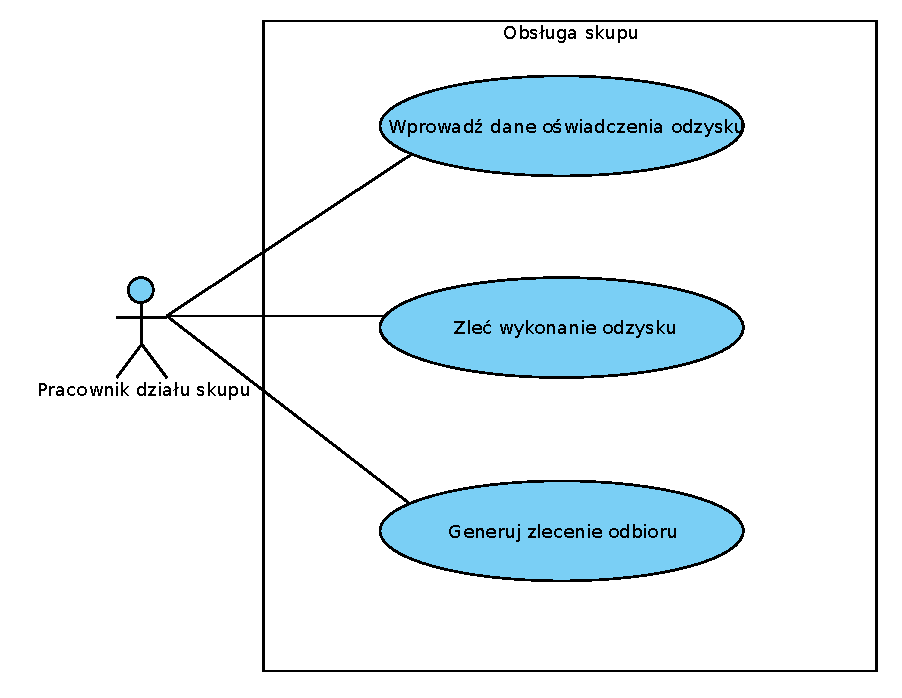
\includegraphics[width=.8\textwidth]{img/UC/skup.eps}
\end{figure}

\begin{usecase}{Generuj zlecenie odbioru na podstawie oferty sprzedaży}
	\textbf{Autor:} Beata Obrok \\
	\textbf{Cel przypadku użycia:} Wysłanie kierowcy do klienta w celu odbioru odpadów \\
	\textbf{Kontekst użycia:} konieczność weryfikacji danych oferty oraz przydzielenia kierowcy do zlecenia \\
	\textbf{Zakres:} System obsługi skupu \\
	\textbf{Poziom:} biznesowy \\
	\textbf{Aktor główny:} Pracownik działu skupu\\
	\textbf{Wyzwalacz:} wybór oferty i wybranie opcji generowania zlecenia \\
	\textbf{Warunek początkowy:} pracownik ma uprawnienia do dodawania zleceń \\
	\textbf{Minimalna gwarancja:} w przypadku niepoprawności danych oferty zlecenie nie zostanie wygenerowane \\
	\textbf{Główny scenariusz powodzenia:} \\
		\begin{enumerate}
			\item Pracownik pozytywnie weryfikuje możliwość wykonania zlecenia
			\item Pracownik zapisuje dane zamawiającego w systemie
			\item Pracownik przydziela kierowcę do zlecenia
			\item Pracownik zapisuje zlecenie w systemie
		\end{enumerate}
	\textbf{Rozszerzenia:} \\
			1.1. Pracownik negatywnie weryfikuje możliwość wykonania zlecenia -> wysyła informację do klienta
\end{usecase}

\begin{figure}[H]
	\centering
	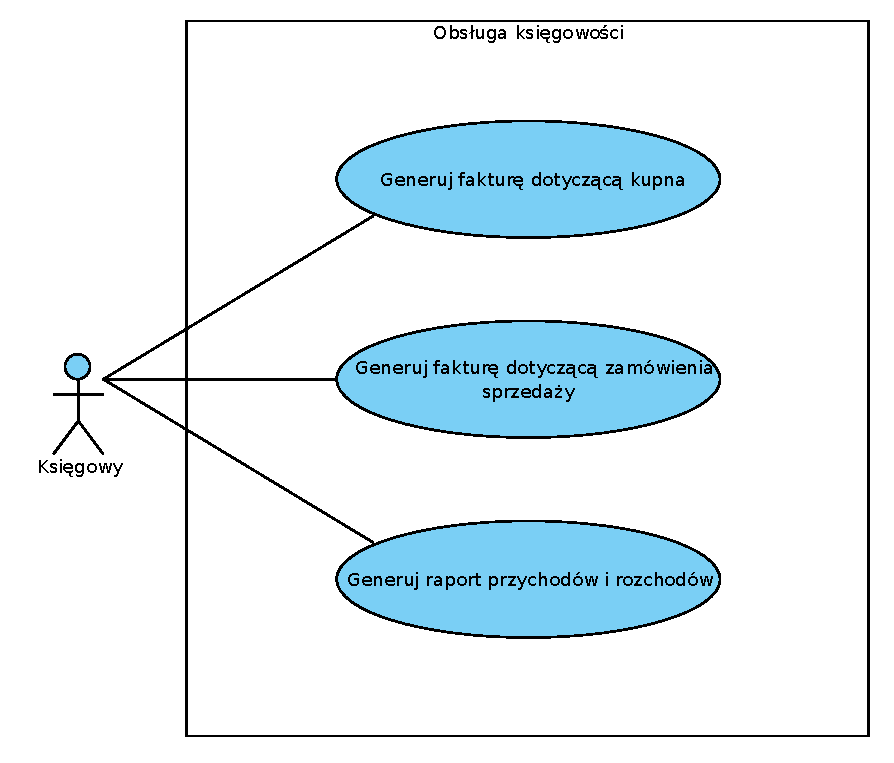
\includegraphics[width=\textwidth]{img/UC/ksiegowosc.eps}
\end{figure}

\begin{usecase}{Generuj fakturę sprzedaży produktów recyklingu}
	\textbf{Autor:} Arkadiusz Socha\\
	\textbf{Cel przypadku użycia:} Wygnerowanie faktury \\
	\textbf{Kontekst użycia:} otrzymanie dokumentu dowodu sprzedaży produktów  \\
	\textbf{Zakres:} system księgujący \\
	\textbf{Poziom:} biznesowy \\
	\textbf{Aktor główny:} Księgowy \\
	\textbf{Wyzwalacz:} sprzedaż produktów recyklingu \\
	\textbf{Warunek początkowy:} księgowy posiada identyfikator zamówienia \\
	\textbf{Minimalna gwarancja:} w przypadku, gdy nie będzie można wygenerować faktury, system poinformuje o tym aktora, nie generując błędnego dokumentu \\
	\textbf{Główny scenariusz powodzenia:} 
		\begin{enumerate}
			\item Księgowy wybiera z listy zamówienie
			\item System upewnie się, czy o to zamówienie chodzi
			\item System generuje fakturę 
		\end{enumerate}
\end{usecase}

\begin{usecase}{Generuj fakturę dotyczącą usługi przejęcia obowiązku recyklingu}
	\textbf{Autor:} Arkadiusz Socha\\
	\textbf{Cel przypadku użycia:} Wygnerowanie faktury \\
	\textbf{Kontekst użycia:} otrzymanie dokumentu dowodu zakupu oświadczenia  \\
	\textbf{Zakres:} system księgujący \\
	\textbf{Poziom:} biznesowy \\
	\textbf{Aktor główny:} Księgowy \\
	\textbf{Wyzwalacz:} kupno oświadczenia oddzysku \\
	\textbf{Warunek początkowy:} księgowy posiada identyfikator danych dotyczących odpowiedniej oferty sprzedaży \\
	\textbf{Minimalna gwarancja:} w przypadku, gdy nie będzie można wygenerować faktury, system poinformuje o tym aktora, nie generując błędnego dokumentu \\
	\textbf{Główny scenariusz powodzenia:} 
		\begin{enumerate}
			\item Księgowy wybiera z listy ofertę sprzedaży
			\item System upewnie się, czy o tą ofertę chodziło
			\item System generuje fakturę 
		\end{enumerate}
\end{usecase}

\begin{usecase}{Wprowadź dane faktury kupna oświadzczenia odzysku}
	\textbf{Autor:} Arkadiusz Socha\\
	\textbf{Cel przypadku użycia:} Wpisanie do systemu danych o fakturze \\
	\textbf{Kontekst użycia:} posiadanie w bazie wszystkich informacji o operacjach firmy\\
	\textbf{Zakres:} system księgujący \\
	\textbf{Poziom:} biznesowy \\
	\textbf{Aktor główny:} Księgowy \\
	\textbf{Wyzwalacz:} kupno oświadczenia oddzysku \\
	\textbf{Warunek początkowy:} księgowy posiada dane o fakturze kupna oświadczenia o przetworzeniu odpadów \\
	\textbf{Minimalna gwarancja:} w przypadku, gdy nie będzie można wproawdzić danych do bazy, nie zostanie ona zmodyfikowana \\
	\textbf{Główny scenariusz powodzenia:} 
		\begin{enumerate}
			\item Księgowy wpisuje dane z faktury do wygenerowanego formularza
			\item System sprawdza czy format poszczególnych danych jest prawidłowy
			\item System wprowadza dane do systemu
		\end{enumerate}
	\textbf{Rozszerzenia:} \\
	2.1 Jeżeli jakieś dane są niepoprawne, księgowy zostaje o tym poinformowany i musi wprowadzić je ponownie
\end{usecase}

\begin{usecase}{Generuj raport przychodów i rozchodów}
	\textbf{Autor:} Arkadiusz Socha\\
	\textbf{Cel przypadku użycia:} Wygnerowanie raportu o zyskach i stratach firmy \\
	\textbf{Kontekst użycia:} otrzymanie raportu dla właściciela  \\
	\textbf{Zakres:} system księgujący \\
	\textbf{Poziom:} biznesowy \\
	\textbf{Aktor główny:} Właściciel \\
	\textbf{Aktor uczestniczący:} Księgowy \\
	\textbf{Wyzwalacz:} właściciel chce mieć informację o przychodach i rozchodach firmy w danym okresie czasowym \\
	\textbf{Warunek początkowy:} podanie ram czasowych  \\
	\textbf{Minimalna gwarancja:} w przypadku, gdy nie będzie można wygenerować raportu, system poinformuje o tym właściciela, nie generując błędnych informacji \\
	\textbf{Główny scenariusz powodzenia:} 
		\begin{enumerate}
			\item Właściciel podaje ramy czasowe okresu, ktory go interesuje
			\item System wybiera tylko te faktury, które zawierają się w podanym przedziale czasowym
			\item System generuje raport
		\end{enumerate}
	\textbf{Rozszerzenia:} \\
	1.1 Ramy czasowe są błędne - conajmniej jedna z wartości jest w przyszłości, system wygeneruje błąd i poprosi o ich ponowne wpisanie
\end{usecase}

\begin{figure}[H]
	\centering
	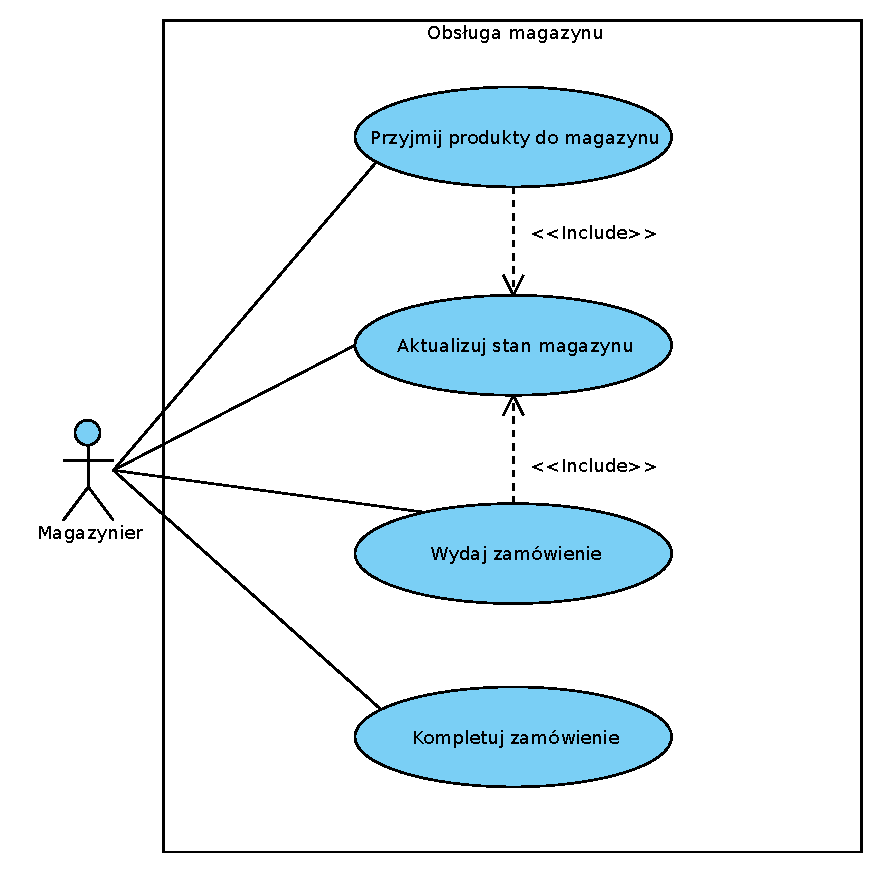
\includegraphics[width=.8\textwidth]{img/UC/magazyn.eps}
\end{figure}

\begin{usecase}{Przyjmij produkty do magazynu}
	\textbf{Autor:} Arkadiusz Socha\\
	\textbf{Cel przypadku użycia:} Dodanie produktów recyklingu do magazynu i aktualizacja stanu magazynu \\
	\textbf{Kontekst użycia:} przechowanie produktów recyklingu w magazynie\\
	\textbf{Zakres:} system magazynowy \\
	\textbf{Poziom:} biznesowy \\
	\textbf{Aktor główny:} Magazynier \\
	\textbf{Uczestnicy:} Kierowca \\
	\textbf{Wyzwalacz:} dostarczenie przez kierowce produktów do magazynu \\
	\textbf{Warunek początkowy:} kierowca ma produkty recyklingu, które należy zmagazynować oraz ich listę \\
	\textbf{Minimalna gwarancja:} w przypadku, gdy produkty nie zostaną zmagazynowane, stan magazynu nie będzie zmieniany \\
	\textbf{Główny scenariusz powodzenia:} \\
		\begin{enumerate}
			\item Kierowca przywozi produkty
			\item Magazynier układa je w magazynie
			\item Magazynier aktualizuje stan magazynu
		\end{enumerate}
\end{usecase}

\begin{usecase}{Wydaj zamówienie}
	\textbf{Autor:} Arkadiusz Socha\\
	\textbf{Cel przypadku użycia:} Wydanie kierowcy produktów, ujętych w zamówieniu \\
	\textbf{Kontekst użycia:} potrzeba przetransporotowania produktów do kupca\\
	\textbf{Zakres:} system magazynowy \\
	\textbf{Poziom:} biznesowy \\
	\textbf{Aktor główny:} Magazynier \\
	\textbf{Uczestnicy:} Kierowca \\
	\textbf{Wyzwalacz:} przyjazd kierowcy do magazynu \\
	\textbf{Warunek początkowy:} kierowca ma zamówienie \\
	\textbf{Minimalna gwarancja:} w przypadku, gdy nie można skompletować zamówienia stan magazynu się nie zmieni \\
	\textbf{Główny scenariusz powodzenia:} 
		\begin{enumerate}
			\item Kierowca przekazuje numer zamówienia magazynierowi
			\item Magazynier wydaje produkty kierowcy
			\item Magazynier uaktualnia stan magazynu
		\end{enumerate}
	\textbf{Rozszerzenia:} \\
	1.1 W przypadku gdy magazynier nie otrzymał wcześniej informacji o zamówieniu, kompletuje je teraz, w razie niepowodzenia produkty nie zostają wydane\\
\end{usecase}

\begin{usecase}{Aktualizuj stan magazynu}
	\textbf{Autor:} Arkadiusz Socha\\
	\textbf{Cel przypadku użycia:} Aktualizacja danych o stanie magayznu \\
	\textbf{Kontekst użycia:} utrzymywanie aktualnej informacji o ilości produktów w magazynie \\
	\textbf{Zakres:} system magazynowy \\
	\textbf{Poziom:} użytkowy \\
	\textbf{Aktor główny:} Magazynier \\
	\textbf{Wyzwalacz:} wydanie lub przyjęcie produktów \\
	\textbf{Warunek początkowy:} zmiana stanu magazynu \\
	\textbf{Minimalna gwarancja:} w przypadku, gdy nie można zaktualizować stanu magazynu, jego stan pozostanie niezmieniony \\
	\textbf{Główny scenariusz powodzenia:} 
		\begin{enumerate}
			\item Magazynier wpisuje informację o wydanych/przyjętych produktach do wygenerowanego formularza
			\item System sprawdza poprawność danych(np. czy magazynier nie wydał więcej niż było w magazynie)
			\item System aktualizje dane
		\end{enumerate}
	\textbf{Rozszerzenia:} \\
	2.1 W przypadku błędnych danych, system informuje o tym magazyniera i prosi o ich ponowne wpisanie\\
\end{usecase}

\begin{usecase}{Kompletuj zamówienie}
	\textbf{Autor:} Arkadiusz Socha\\
	\textbf{Cel przypadku użycia:} Skompletowanie zamówienie w celu wydania go kierowcy \\
	\textbf{Kontekst użycia:} chęć uporządkowania produktów do zamówienia w celu szybkiego ich przekazania kierowcy \\
	\textbf{Zakres:} system magazynowy \\
	\textbf{Poziom:} biznesowy \\
	\textbf{Aktor główny:} Magazynier \\
	\textbf{Wyzwalacz:} dostanie informacji o zamówieniu \\
	\textbf{Warunek początkowy:} odpowiednia ilość towarów w magazynie \\
	\textbf{Minimalna gwarancja:} w przypadku, gdy nie ma odpowiedniej ilości towarów w magazynie, zostanie wysłana informacja zwrotna  \\
	\textbf{Główny scenariusz powodzenia:} 
		\begin{enumerate}
			\item Magazynier otrzymuje listę towarów, które wchodzą w skład zamówienia
			\item Magazynier sprawdza czy posiada ich odpowiednią ilość
			\item Magazynier przygotowuje zamówienie
		\end{enumerate}
	\textbf{Rozszerzenia:} \\
	2.2. Nie można skompletować zamówienia, zostaje wysłana informacja zwrotna o nieposiadanych towarach\\
\end{usecase}

\begin{figure}[H]
	\centering
	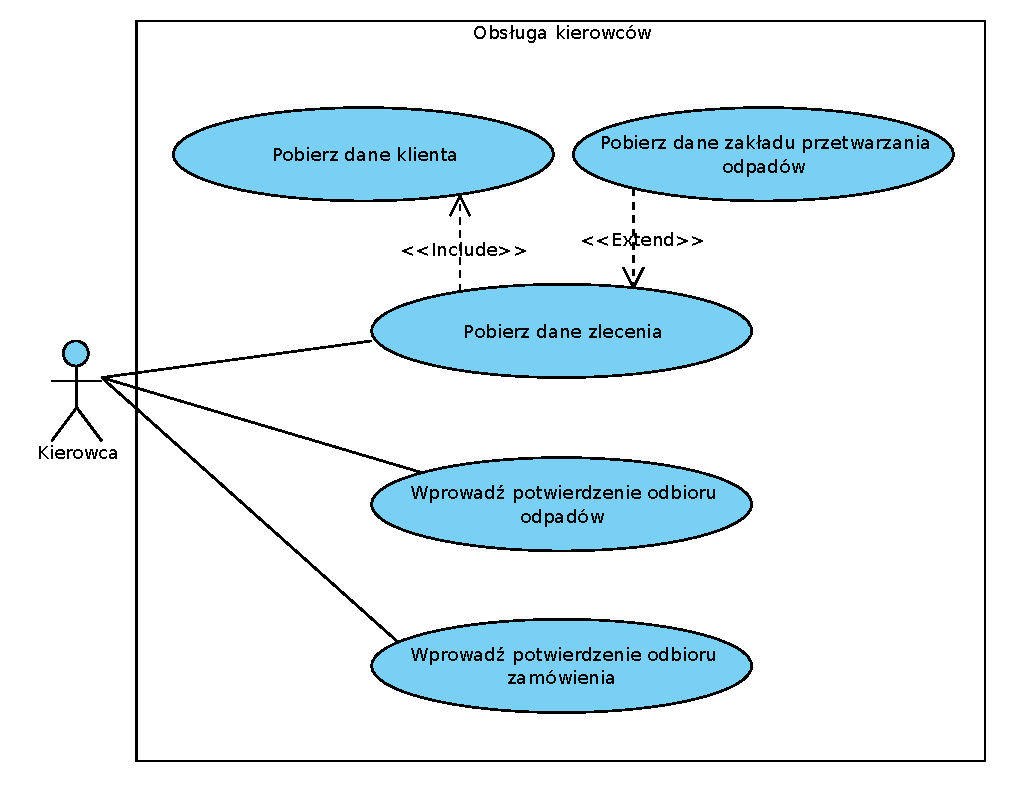
\includegraphics[width=.8\textwidth]{img/UC/kierowcy.eps}
\end{figure}

%TODO
\begin{usecase}{Pobierz dane zlecenia}
	\textbf{Autor:} Beata Obrok\\
	\textbf{Cel przypadku użycia:} \\
	\textbf{Kontekst użycia:} \\
	\textbf{Zakres:} Obsługa kierowców \\
	\textbf{Poziom:} biznesowy \\
	\textbf{Aktor główny:} Kierowca \\
	\textbf{Wyzwalacz:}  \\
	\textbf{Warunek początkowy:}  \\
	\textbf{Minimalna gwarancja:} \\
	\textbf{Główny scenariusz powodzenia:} 
		\begin{enumerate}
			\item 
		\end{enumerate}
	\textbf{Rozszerzenia:} \\
\end{usecase}

%TODO
\begin{usecase}{Wprowadź potwierdzenie odbioru odpadów}
	\textbf{Autor:} Beata Obrok\\
	\textbf{Cel przypadku użycia:} \\
	\textbf{Kontekst użycia:} \\
	\textbf{Zakres:} Obsługa kierowców \\
	\textbf{Poziom:} biznesowy \\
	\textbf{Aktor główny:} Kierowca \\
	\textbf{Wyzwalacz:}  \\
	\textbf{Warunek początkowy:}  \\
	\textbf{Minimalna gwarancja:} \\
	\textbf{Główny scenariusz powodzenia:} 
		\begin{enumerate}
			\item 
		\end{enumerate}
	\textbf{Rozszerzenia:} \\
\end{usecase}

%TODO
\begin{usecase}{Wprowadź potwierdzenie odbioru zamówienia}
	\textbf{Autor:} Beata Obrok\\
	\textbf{Cel przypadku użycia:} \\
	\textbf{Kontekst użycia:} \\
	\textbf{Zakres:} Obsługa kierowców \\
	\textbf{Poziom:} biznesowy \\
	\textbf{Aktor główny:} Kierowca \\
	\textbf{Wyzwalacz:}  \\
	\textbf{Warunek początkowy:}  \\
	\textbf{Minimalna gwarancja:} \\
	\textbf{Główny scenariusz powodzenia:} 
		\begin{enumerate}
			\item 
		\end{enumerate}
	\textbf{Rozszerzenia:} \\
\end{usecase}

	\subsection{Wymagania funkcjonalne dla dodatkowych funkcji systemu}
		% funkcje administracyjne, wspólne i wewnętrzne
		
\begin{enumerate}
\item Funkcje administracyjne
	\begin{itemize}
		\item użytkownik systemu z uprawnieniami administratora (administrator) może dodawać i usuwać pracowników za pomocą panelu administracyjnego (nadawać użytkownikom określone uprawnienia, niezbędne do wykonywania ich pracy z systemem)
		\item administrator ma dostęp do wszystkich deklaracji
		\item po nadaniu deklaracji statusu „przyjętej” zmian w niej może dokonywać tylko administrator na wniosek klienta
	\end{itemize}

\item Funkcje wspólne
	\begin{itemize}
		\item użytkownik może edytować deklarację do momentu nadania jej statusu „przyjętej”
		\item zależnie od uprawnień użytkownik systemu może pobrać swoje wszystkie zarchiwizowane deklaracje w wygodnym dla niego pliku
		\item użytkownik może sprawdzić stan danej przesyłki odpadów
	\end{itemize}

\item Funkcje wewnętrzne
	\begin{itemize}
		\item generowanie faktur
		\item generowanie potwierdzeń odbioru dla kierowców
		\item tworzenie kopii zapasowych
		\item pobieranie danych archiwalnych
	\end{itemize}

\end{enumerate}

	\subsection{Wymagania niefunkcjonalne}
		% z podziałem na grupy wymagań
		
\begin{enumerate}
\item Użyteczność
	\begin{itemize}
		\item interakcja z użytkownikiem powinna być czytelna
		\item użycie prostych, estetycznych i czytelnych czcionek
		\item użycie intuicyjnych kolorów, np. dla błędnych danych koloru czerwonego
		\item w miarę możliwości składanie deklaracji powinno być analogiczne do wypełniania innych formularzy internetowych
		\item bez zbyt złożonych efektów wizualnych, które będą widocznie spowalniały działanie systemu na słabszym sprzęcie
	\end{itemize}

\item Niezawodność
	\begin{itemize}
		\item czas awarii nie może być dłuższy niż dwie godziny
		\item każdy użytkownik ma dostęp do systemu z określonymi, niezbędnymi uprawnieniami
	\end{itemize}

\item Wydajność
	\begin{itemize}
		\item system będzie w stanie dodać nową deklarację w mniej niż 5s
		\item system będzie w stanie wygenerować nową fakturę w mniej niż 5s
		\item system wyeksportuje dane archiwalne o wielkości do 100 mb w mniej niż 10s
	\end{itemize}

\item Wspieralność
	\begin{itemize}
		\item system powinien być skalowalny, tj. dodanie nowej funkcji przetwarzania/przedstawienia danych podanych przez klienta nie powinno powodować zmiany wcześniej napisanego kodu
		\item system napisany będzie w języku Java
		\item strona internetowa będzie używała języka JavaScript


\item Harmonogram
	\begin{itemize}
		\item I miesiąc - analiza wymagań
		\item II, III miesiąc - projekt wstępny
		\item IV - VII miesiąc - projekt szczegółowy
		\item VIII - XII miesiąc - implementacja
	\end{itemize}


\end{enumerate}

\section{Analiza funkcjonalna systemu}

	\subsection{Diagram kontekstowy}
		
\begin{figure}[H]
	\centering
	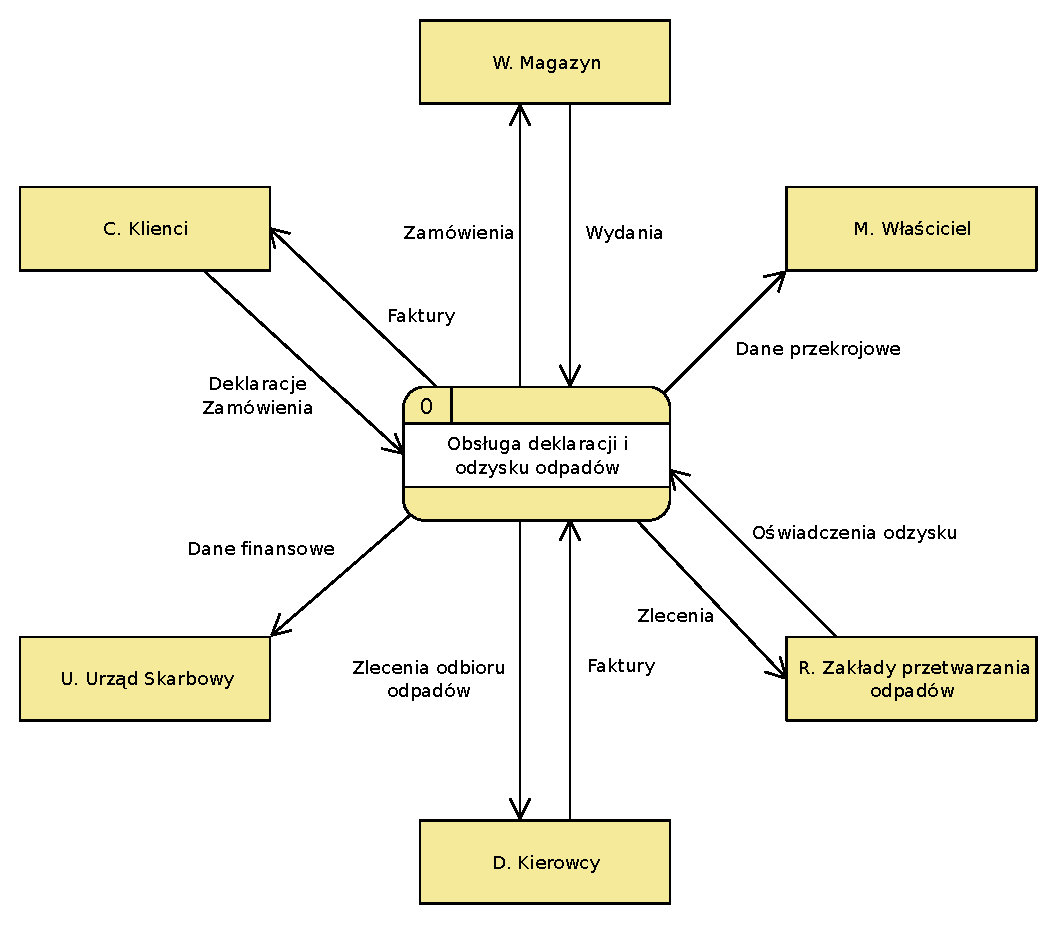
\includegraphics[width=\textwidth]{img/DFD/context.eps}
\end{figure}

	\subsection{Analiza top-down}
		\begin{landscape}
	\subsubsection{Poziom 1}
		\begin{figure}[H]
			\centering
			\centerline{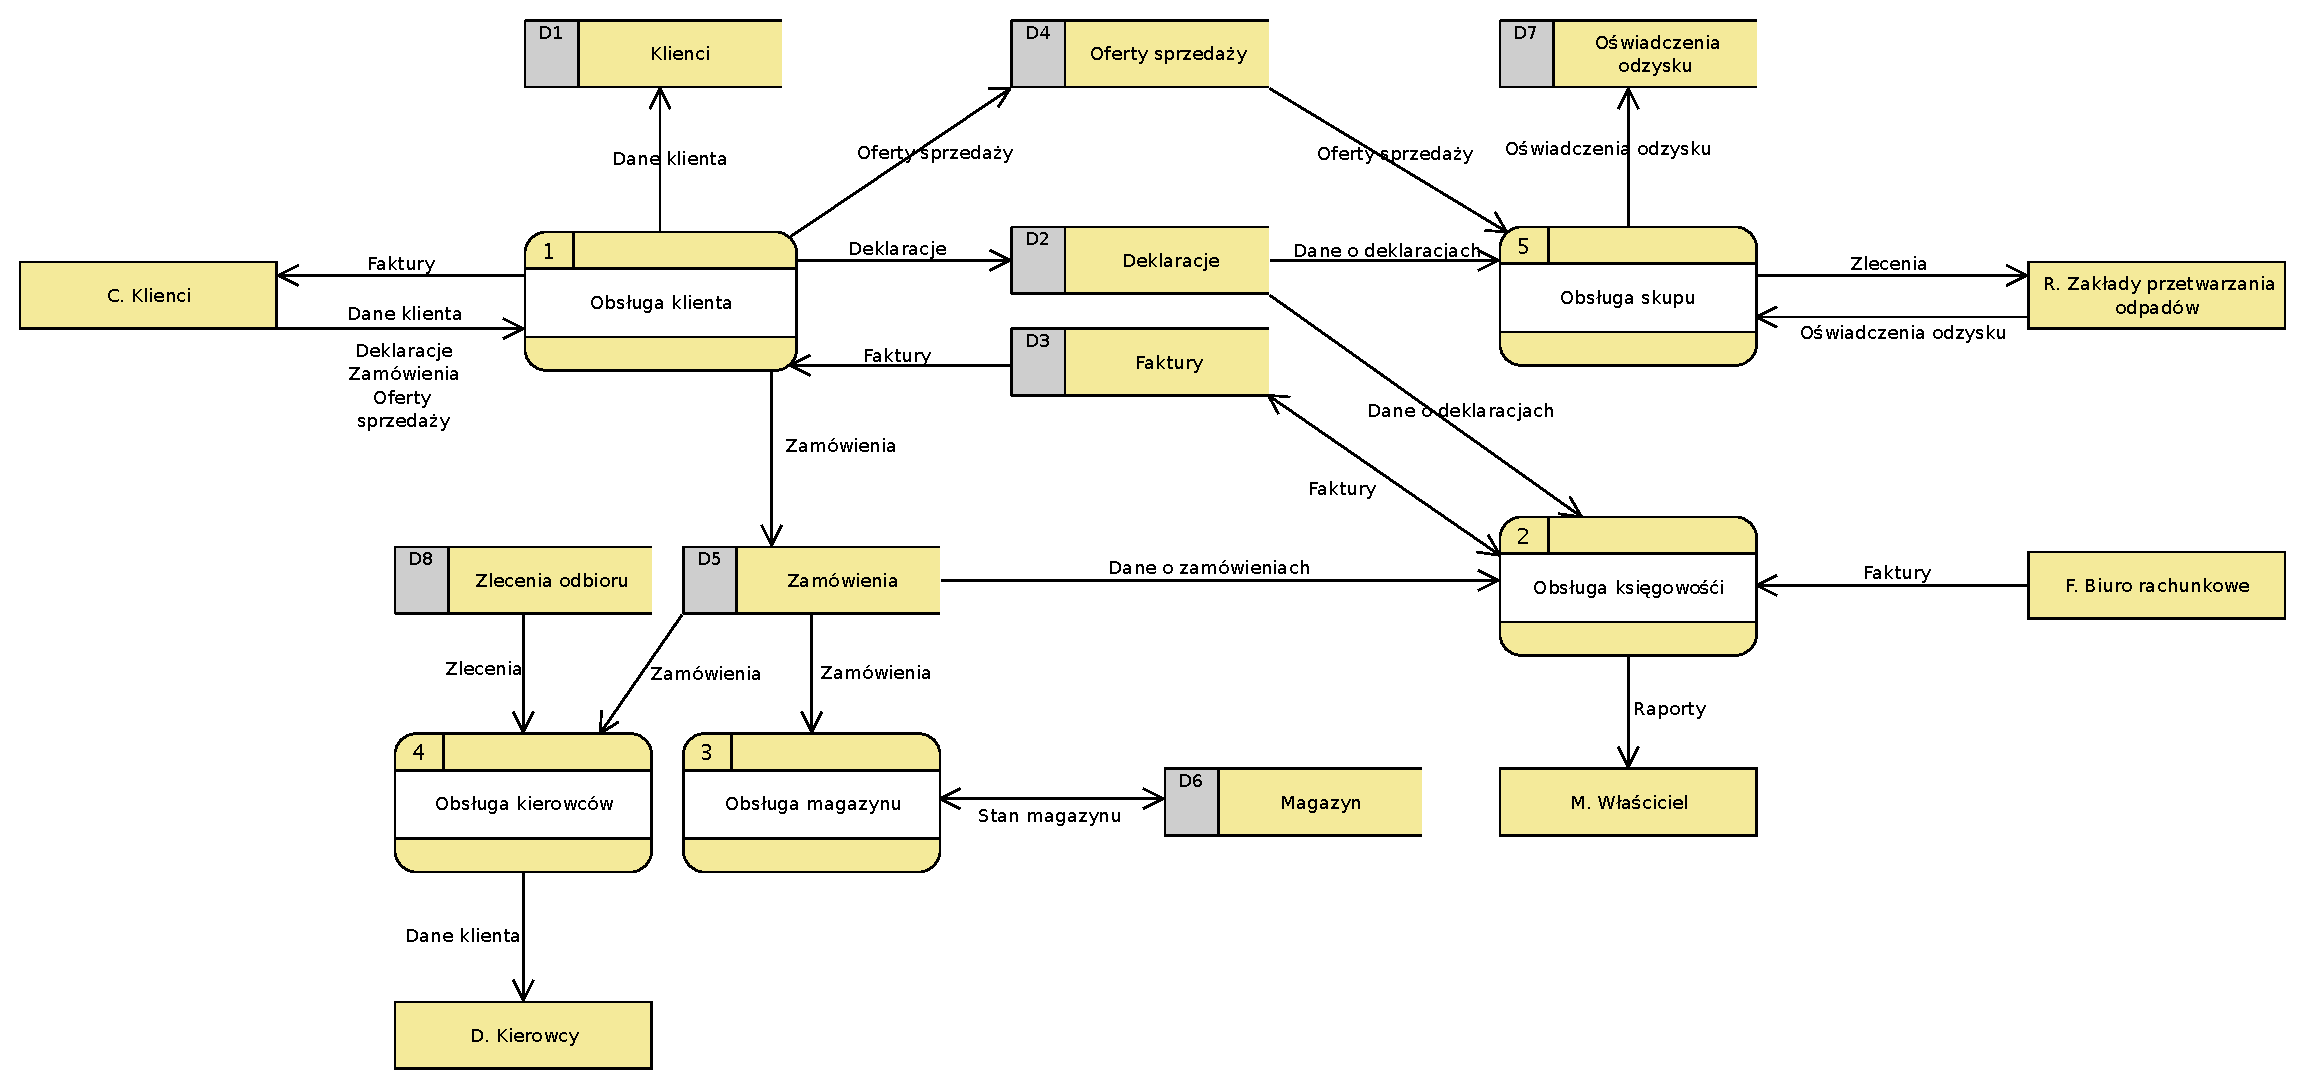
\includegraphics[width=29cm]{img/DFD/1-level.eps}}
		\end{figure}
\end{landscape}

	%DFD1
	\textbf{Opis}\\
	Digram pokazuje wyodrębnienie podsystemów, które są przedstawione bardziej szczegółowo na kolejnych diagramach.

\subsubsection{Poziom 2}
	%DFD2 - Obsługa magazynu
	\begin{figure}[H]
		\centering
		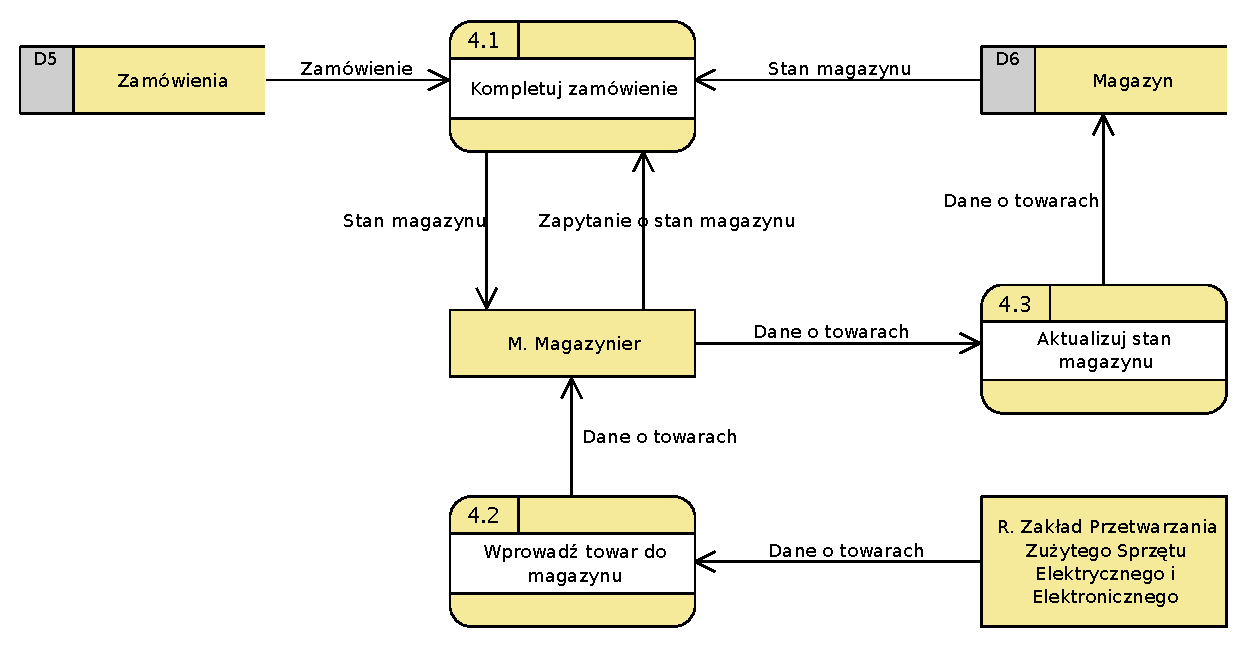
\includegraphics[width=\textwidth]{img/DFD/2-level-magazyn.eps}
		\caption{Obsługa magazynu}
	\end{figure}

	\textbf{Opis} \\
	\underline{3.1 Kompletuj zamówienie}\\
	Magazynier pyta o stan magazynu, aby sprawdzić, czy może skompletować zamówienie.
	\textbf{Strumień wejściowy} zapytanie o stan magazynu, zamówienie\\
	\textbf{Strumień wyjściowy} aktualny stan magazynu\\

	\underline{3.2 Aktualizuj stan magazynu}\\ 
	Stan magazynu jest aktualizowany na podstawie ilości produktów dostarczanych lub odbieranych.\\	
	\textbf{Strumień wejściowy} Produkty przyjmawane do magazynu, produkty wydawane przez magazyn.\\
	\textbf{Strumień wyjściowy} Produkty przyjmawane do magazynu, produkty wydawane przez magazyn.\\
	\underline{3.3 Wprowadź towar do magazynu}\\
	Towar zostaje przywieziony przez kierowcę z Zakładu Przetwarzania Zużytego Sprzętu Elektrycznego i Elektronicznego, informacje o jego ilości są zapisywane do systemu.\\
	\textbf{Strumień wejściowy} Dane o przywiezionych towarach\\
	\textbf{Strumień wyjściowy} Dane o przywiezionych towarach



	\begin{figure}[H]
		\centering
		\centerline{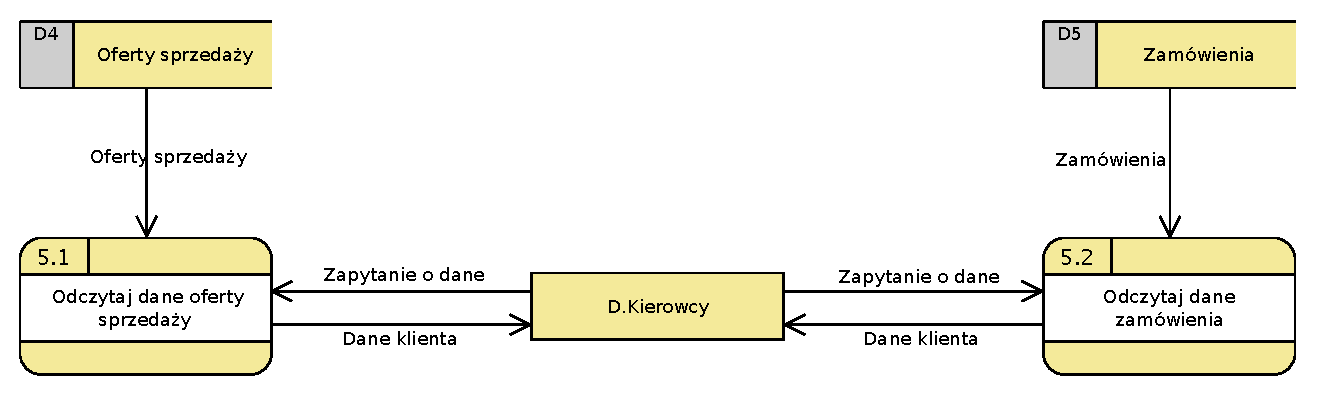
\includegraphics[width=1.1\textwidth]{img/DFD/2-level-kierowcy.eps}}
		\caption{Obsługa kierowców}
	\end{figure}

	\begin{figure}[H]
		\centering
		\centerline{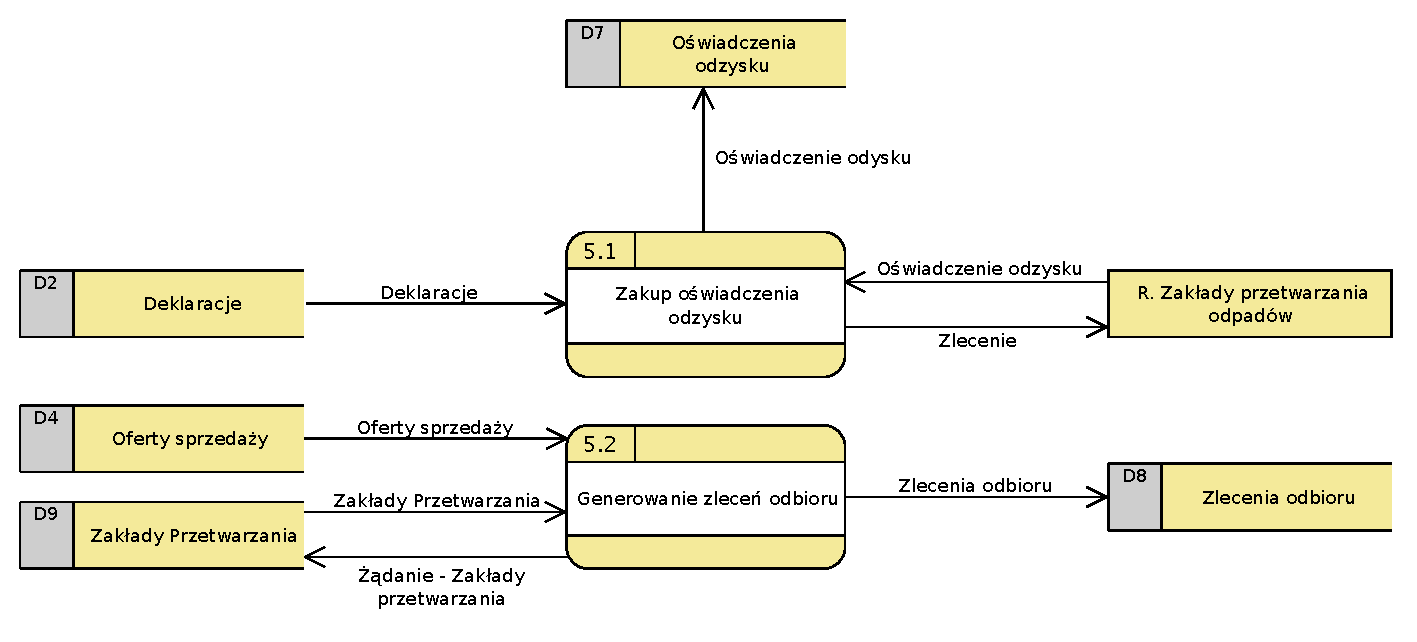
\includegraphics[width=1.1\textwidth]{img/DFD/2-level-skup.eps}}
		\caption{Obsługa skupu}
	\end{figure}

	\begin{figure}[H]
		\centering
		\centerline{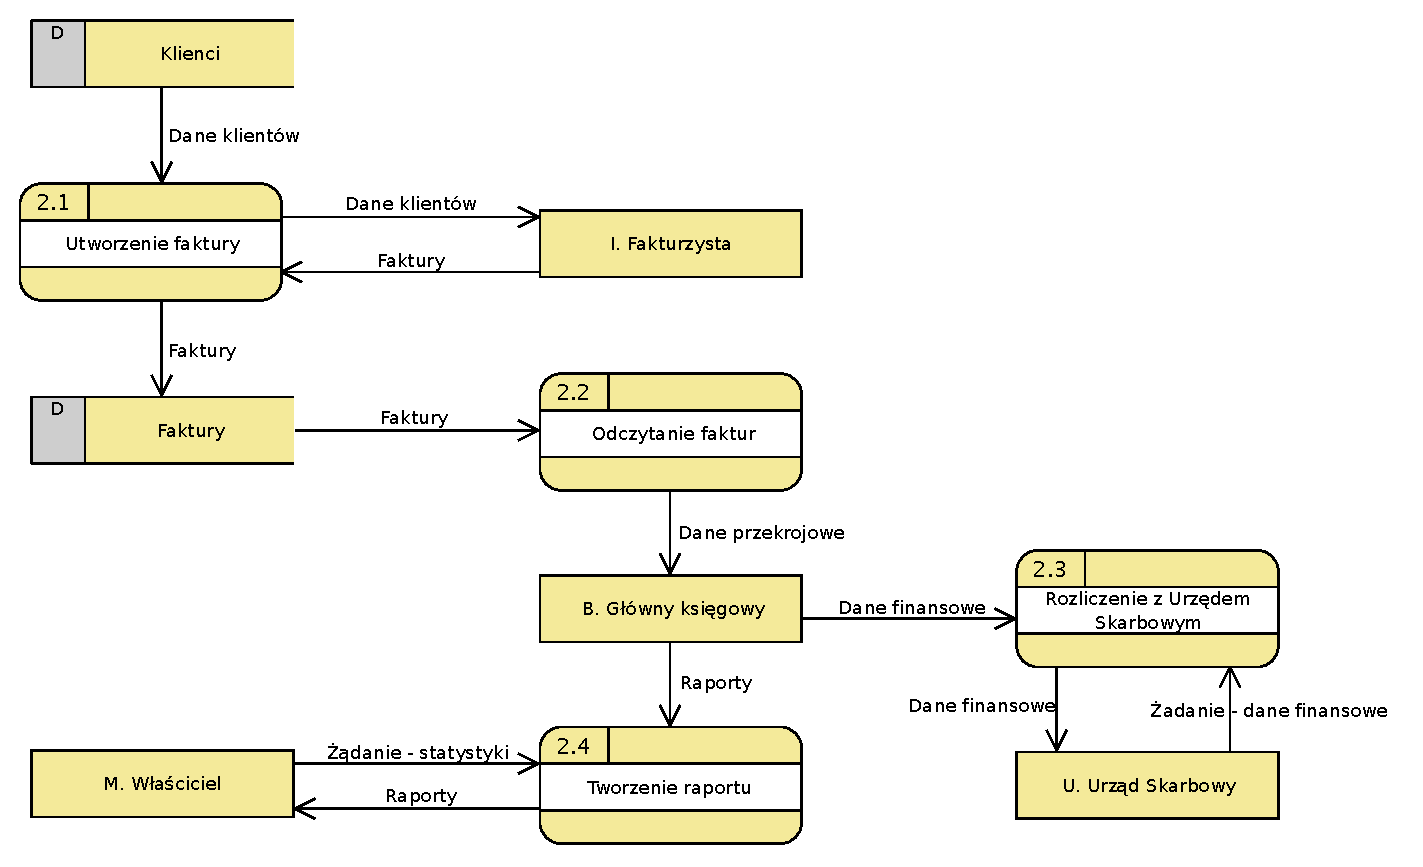
\includegraphics[width=1.1\textwidth]{img/DFD/2-level-ksiegowosc.eps}}
		\caption{Obsługa księgowości}
	\end{figure}

	\subsection{Opis procesów}
		\input{partials/3-analiza/3-procesy.tex}

% \section{Roboczy słownik danych}

\section{Analiza struktur danych w przechowywanych magazynach}
	
\begin{figure}
	\centering
	\vspace{-2cm}
	\centerline{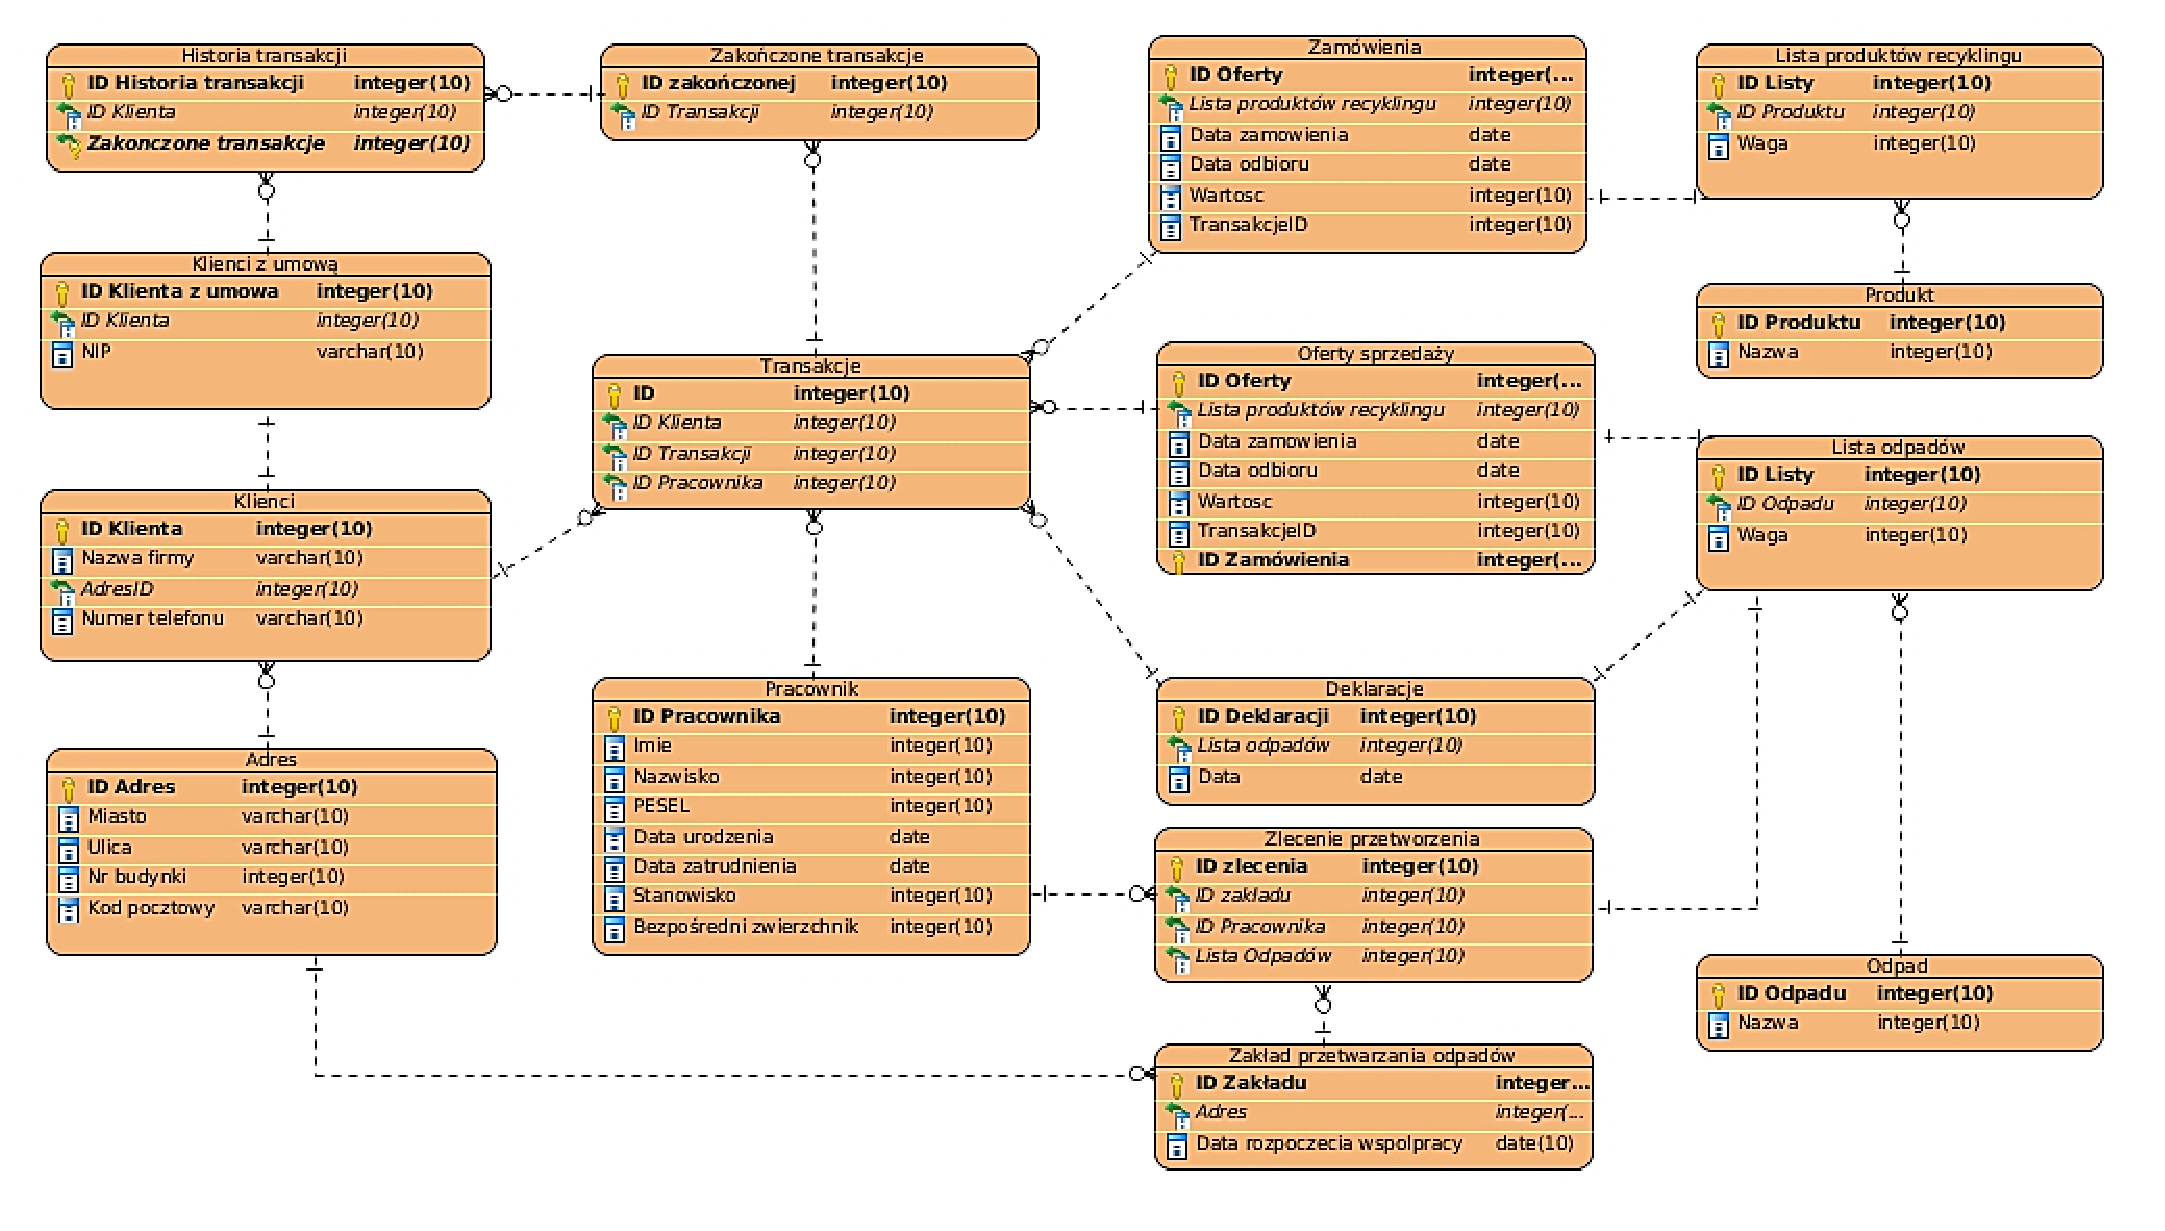
\includegraphics[angle=90, height=29cm]{img/ERD.eps}}
\end{figure}

% \section{Obraz zachowania systemu w czasie}

% \section{Równoważenie modeli}

% \section{Architektura systemu}

% 	\subsection{Architektura całego systemu}

% 	\subsection{Architektura podsystemów}

% 	\subsection{Wewnętrzna architektura podsystemów}

% \section{Projekt interfejsu użytkownika}

% \section{Podsumowanie}

% 	\subsection{Założenia implementacyjne}

% 	\subsection{Weryfikacja projektu systemu}

% 	\subsection{Uwagi i wnioski końcowe}

%%% End document

\section{Słownik}
	\paragraph{Klient} \ \\
Firma, dla której BIOSYSTEM świadczy usługi przejęcia obowiązku odzysku odpadów.

\paragraph{Klient bez konta} \ \\
Firma lub osoba prywatna, który może zamówić odbiór odpadów za pomocą projektowanego systemu.

\paragraph{Deklaracja} \ \\
Dokument składany przez \emph{Klienta} dotyczący wprowadzonych do obiegu przez \emph{Klienta} odpadów oraz ich ilości.

\paragraph{Oświadczenie odzysku} \ \\
Dokument kupowany od \emph{Zewnętrznych Zakładów Przetwarzających Odpady}, który opisuje rodzaje odzyskanych odpadów oraz ich ilości.
Jest on wymagany przez Ustawę o Odzysku.

\paragraph{Zewnętrzny Zakład Przetwarzający Odpady}
Firma niezwiązana z firmą BIOSYSTEM przeprowadzająca odzysk odpadów.


\section{Załączniki}
	\subsection{Dokumenty wprowadzane i wyprowadzane z systemu}
		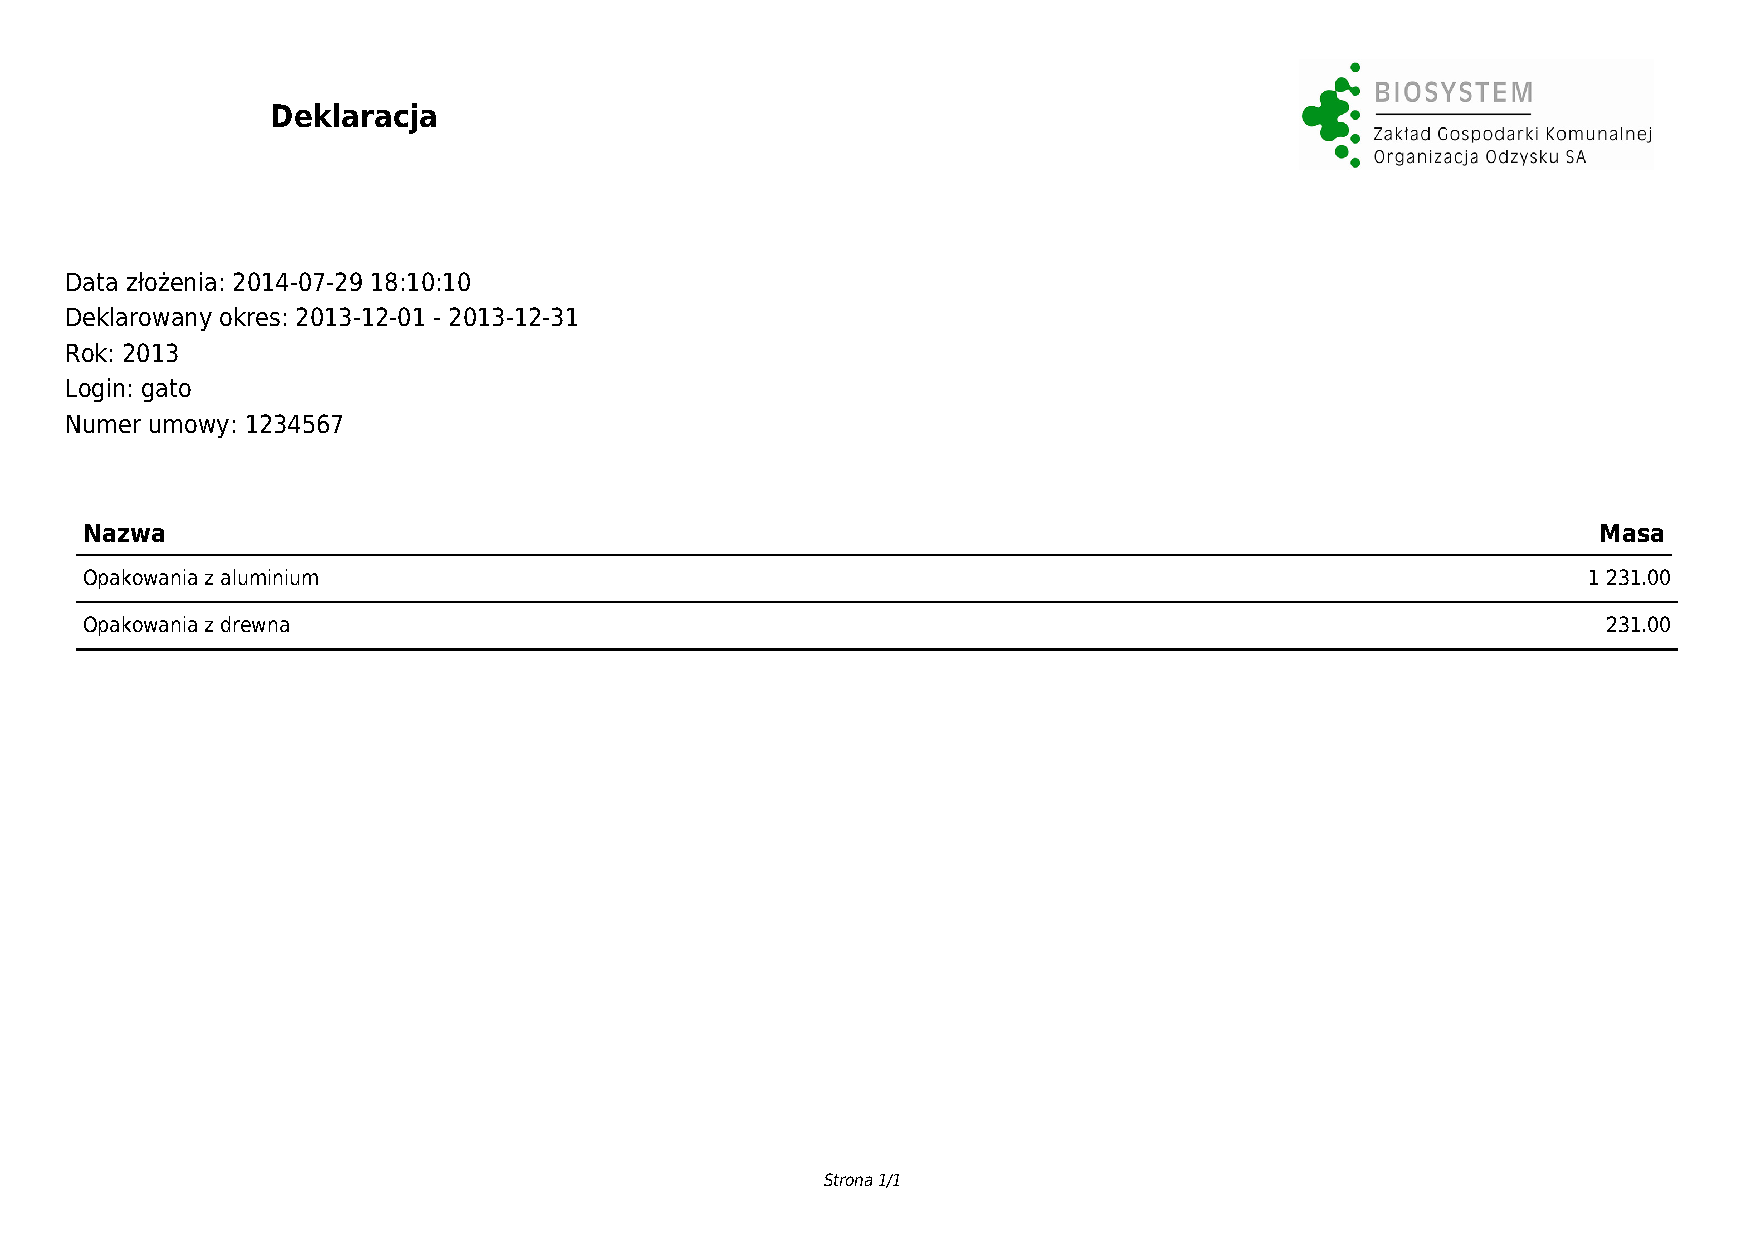
\includepdf[pages={1}, angle=90]{partials/2-wymagania/dokumenty/deklaracja.pdf}
		\begin{figure}[H]
			\centering
			\vspace{-2cm}
			\centerline{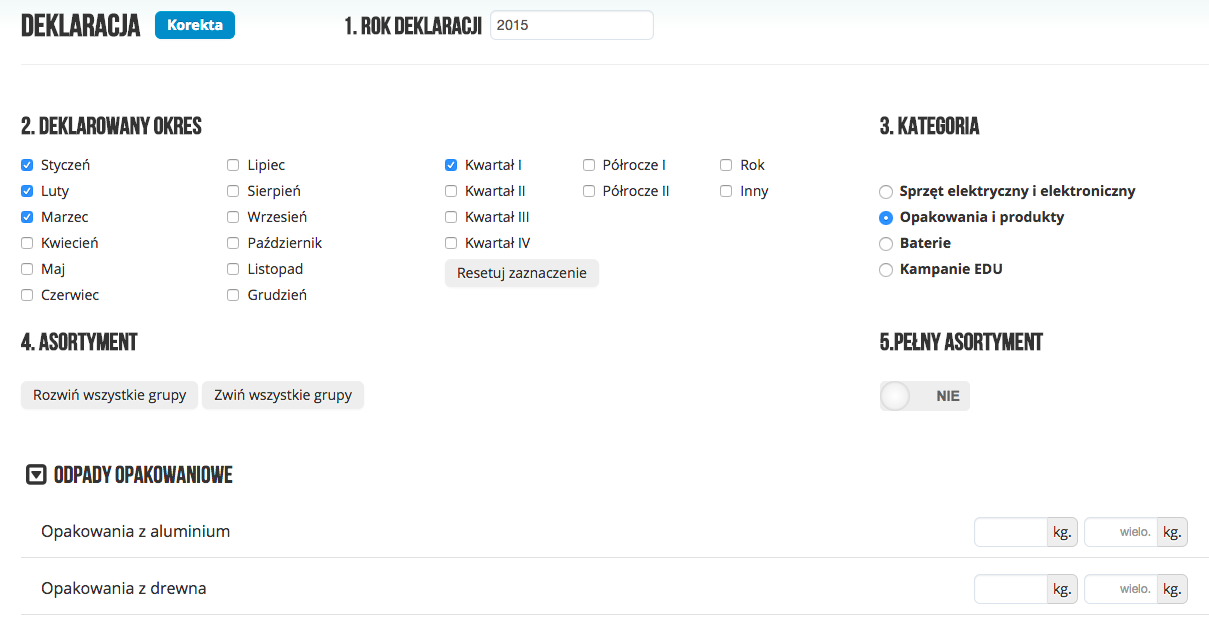
\includegraphics[angle=90, height=29cm]{partials/2-wymagania/dokumenty/formularz.png}}
		\end{figure}
		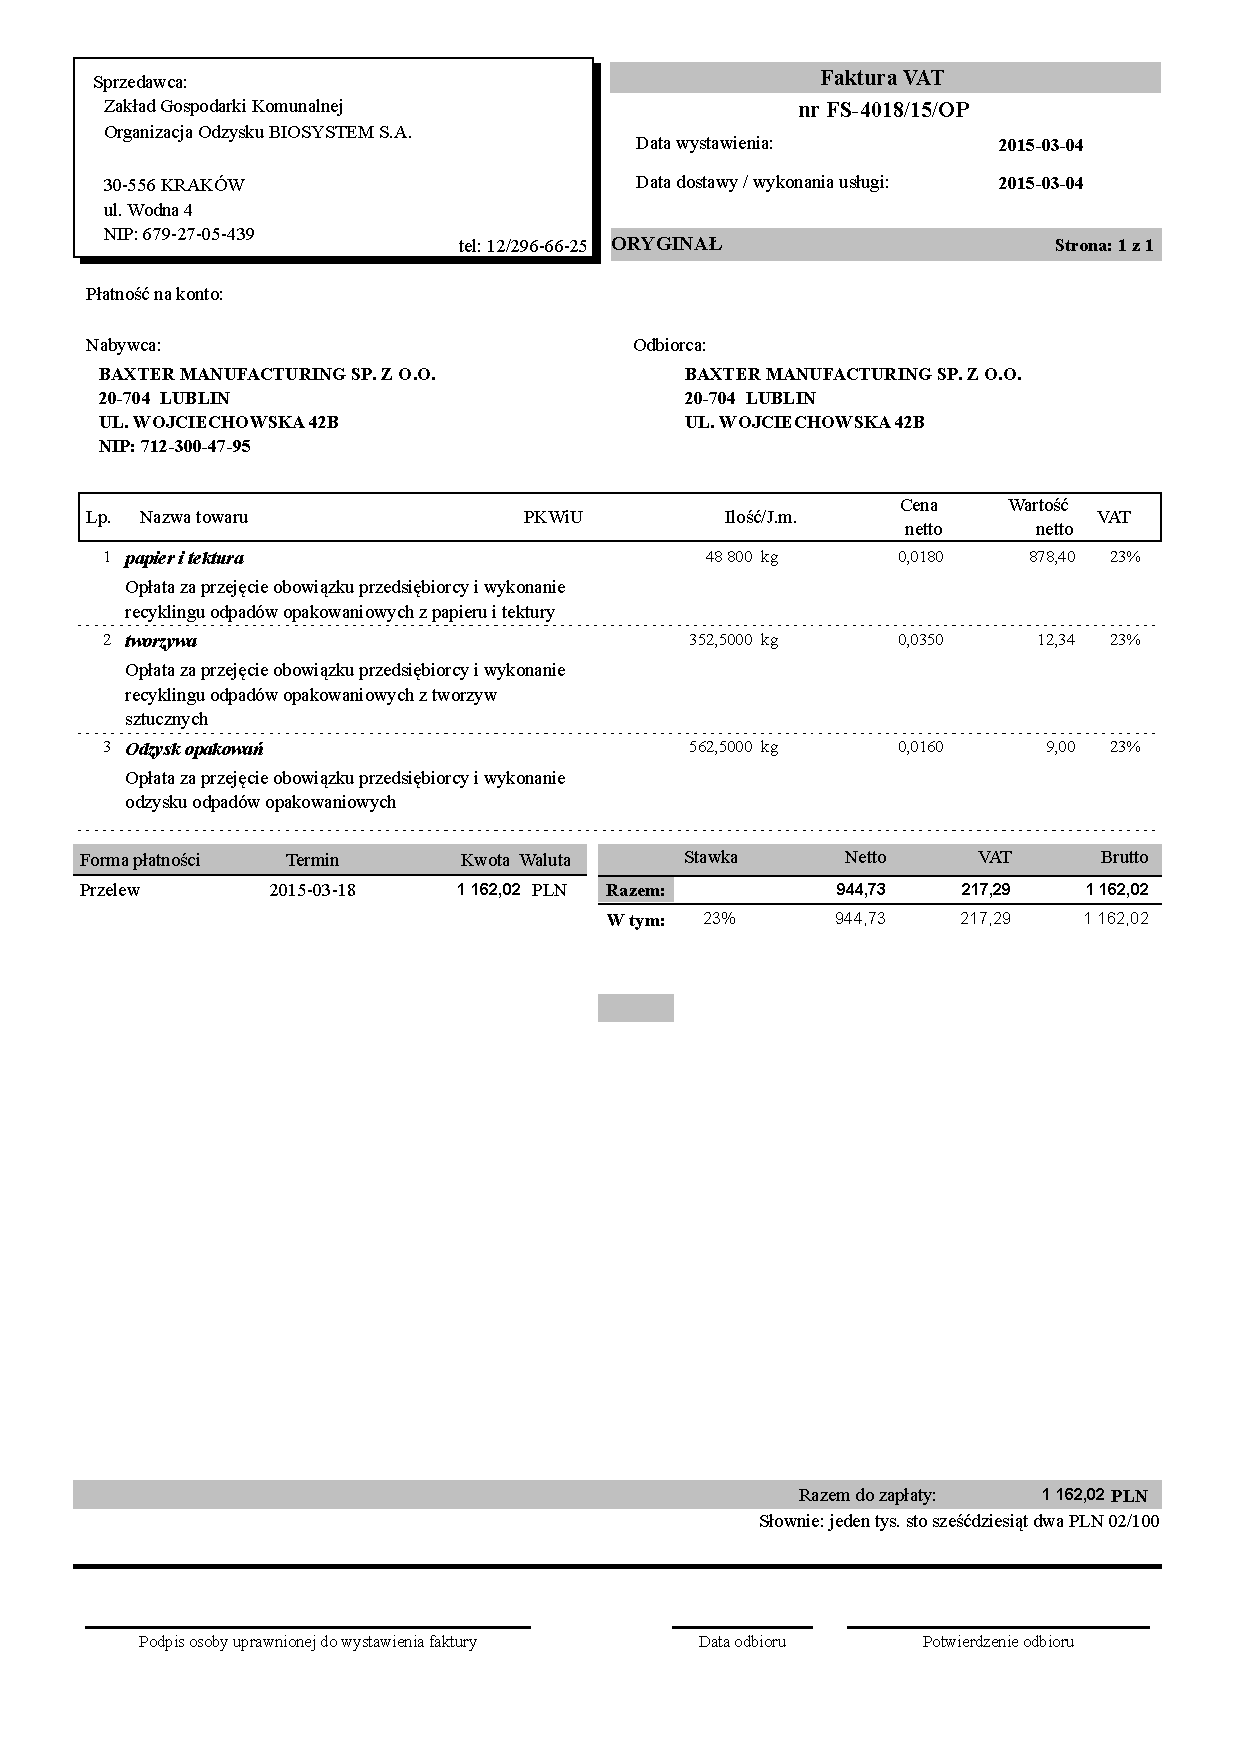
\includepdf[pages={1}]{partials/2-wymagania/dokumenty/faktura.pdf}
\end{document}